\documentclass[aspectratio=169, xcolor=table]{beamer}
\usepackage[english,russian]{babel}
\usepackage[utf8]{inputenc}
\usepackage{multicol}
\usepackage{tabularx}
\usepackage{wasysym}
%\usepackage[table,xcdraw]{xcolor} % чтобы красить таблички

%biblatex-gost
\usepackage[backend=biber, style=gost-authoryear, bibstyle=gost-authoryear, language=auto, babel=other, bibencoding=utf8, bibdoi=false, biburl=false,  movenames=false, sortcites = false]{biblatex}
\addbibresource{../txt/sophia_base.bib}

\mode<presentation>
%\mode<article>
% Стиль презентации
%\usetheme{Warsaw}
% \usetheme{Madrid}
\usetheme{Marburg}
%\usetheme{Hannover}
%\usetheme{Singapore}
%\usecolortheme{seahorse}



% в начале каждого раздела печатаем содержание с выделением текущего раздела
%\AtBeginSection[]
%{
%  \begin{frame}<beamer>{Содержание}
%    \tableofcontents[currentsection]
%  \end{frame}
%}

%\beamertemplatenavigationsymbolsempty
\setbeamertemplate{navigation symbols}{\insertslidenavigationsymbol, \insertsectionnavigationsymbol, \insertdocnavigationsymbol}

%\setbeamerfont{page number in head/foot}{size=\large}
%\setbeamertemplate{footline}[frame number]



\begin{document}

\title[]{ОРГАНИЗАЦИЯ ПОСЕЛЕНИЙ\\ {\it Macoma~balthica}~(Linnaeus,~1758)\\ В ОСУШНОЙ ЗОНЕ БЕЛОГО И БАРЕНЦЕВА МОРЕЙ}
\author[]{София Александровна Назарова \\ \medskip
	\footnotesize{Научный руководитель: д.б.н.~Н.~В.~Максимович}}
\institute[СПбГУ]{Санкт-Петербургский государственный университет}
\date{Санкт-Петербург, 2016} 

% Создание заглавной страницы
{\usebackgroundtemplate{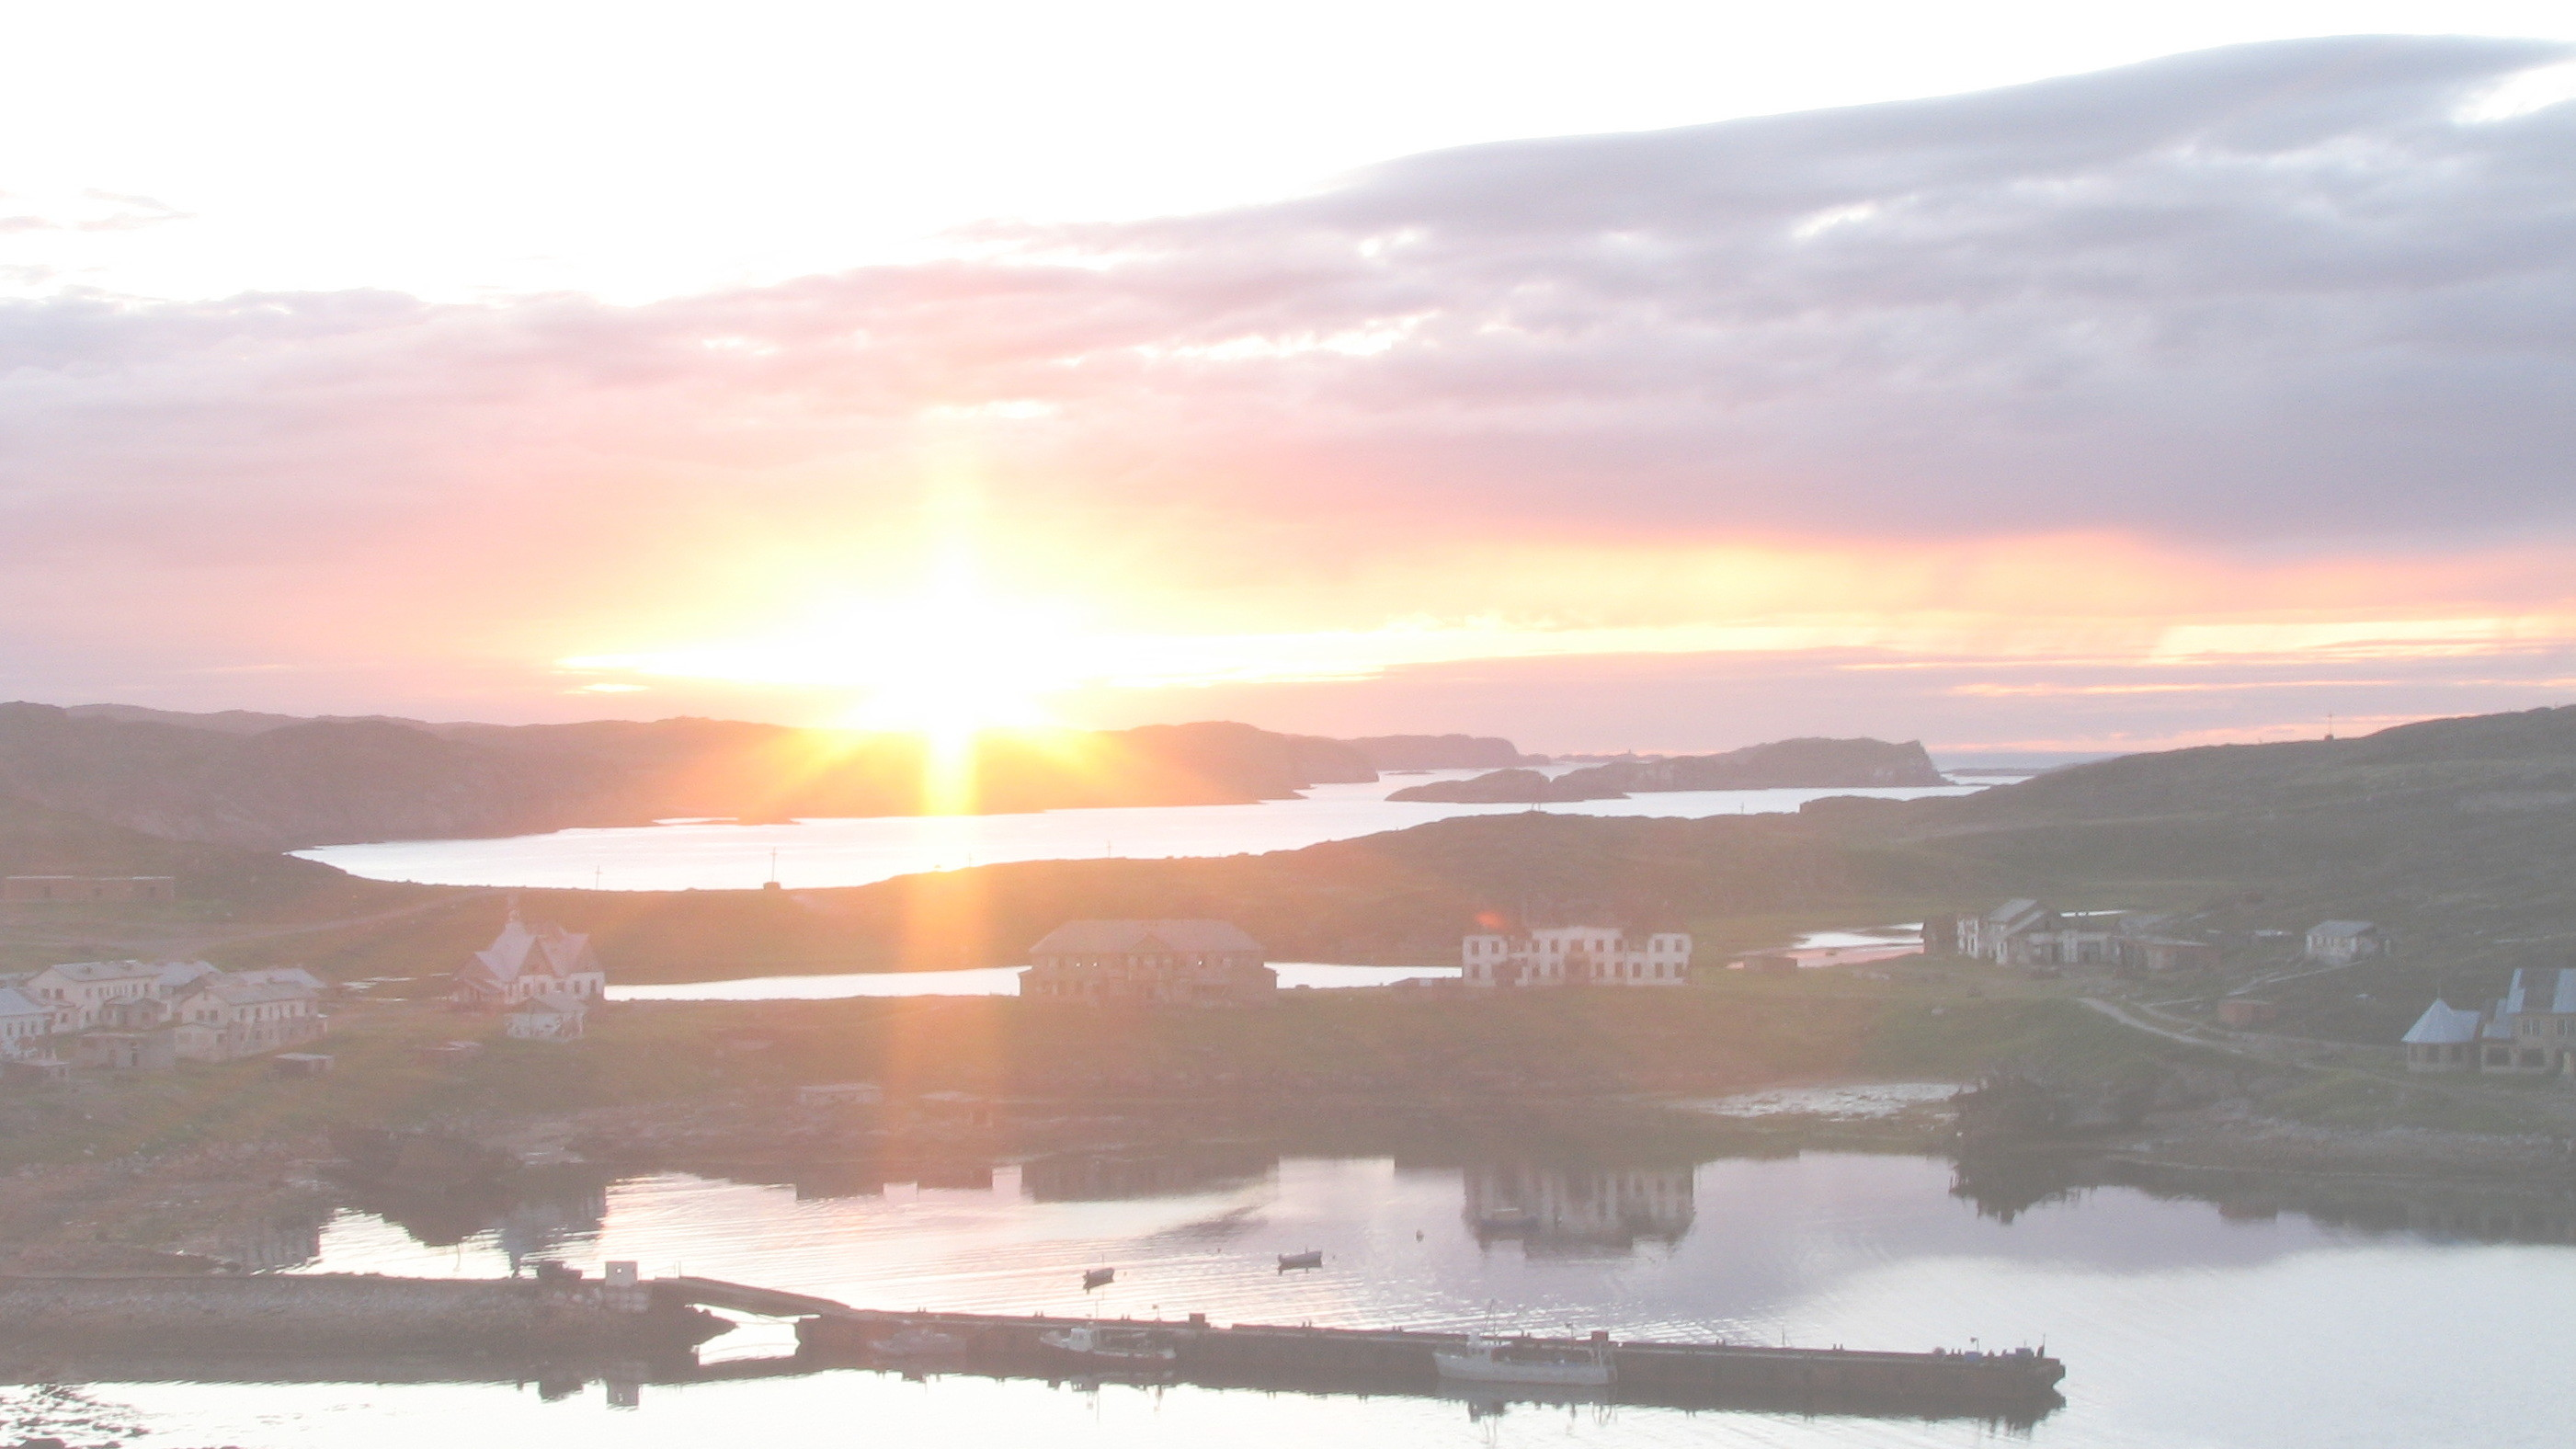
\includegraphics[width=\paperwidth]{fon.JPG}}
\frame{\titlepage} 
}





%%%%%%%%%%%%%%%%%%%%%%%%%%%%%%%%%%%%%%%%%%%%%%%%%%%%%
		\section{Введение}
%%%%%%%%%%%%%%%%%%%%%%%%%%%%%%%%%%%%%%%%%%%%%%%%%%%%%
\begin{frame}{\insertpagenumber.\ Вид {\it Macoma~balthica} (Linnaeus, 1758)}

{\scriptsize Общий вид особей}
			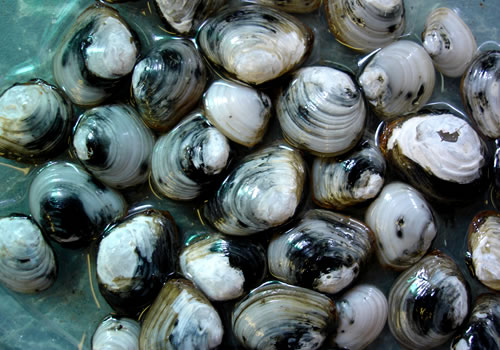
\includegraphics[width=.4\textwidth]{Baltic_macoma.jpg}	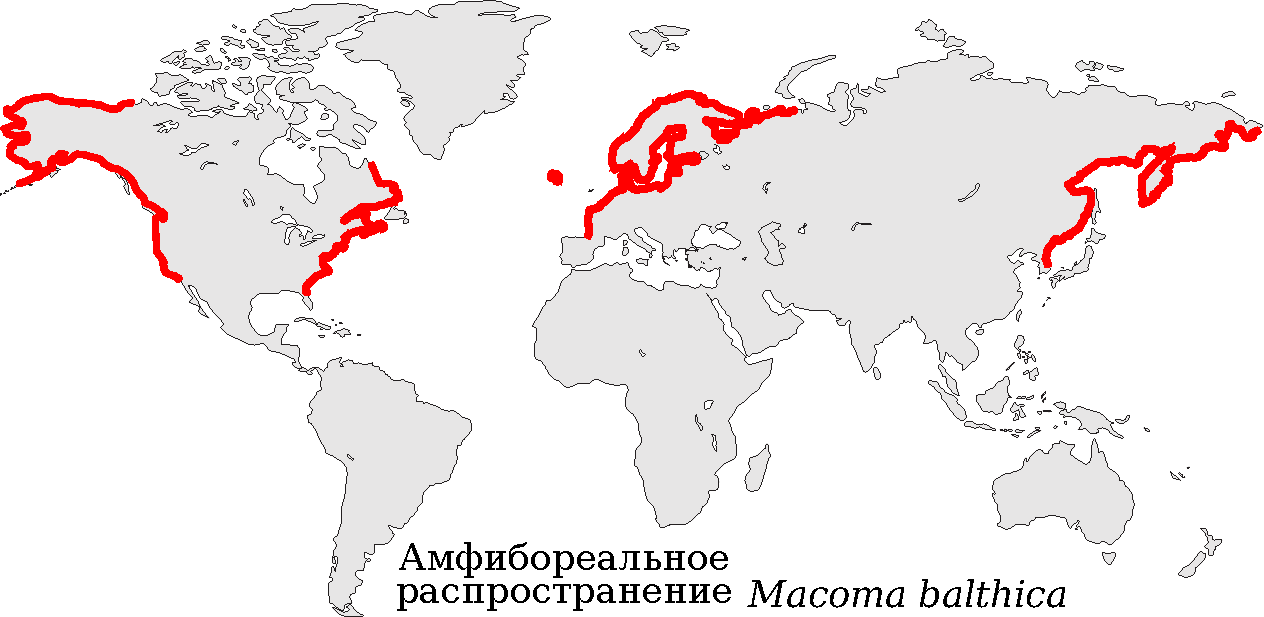
\includegraphics[width=.6\textwidth]{areal_line.pdf}

{\scriptsize Типичные местообитания в Белом и Баренцевом море}
			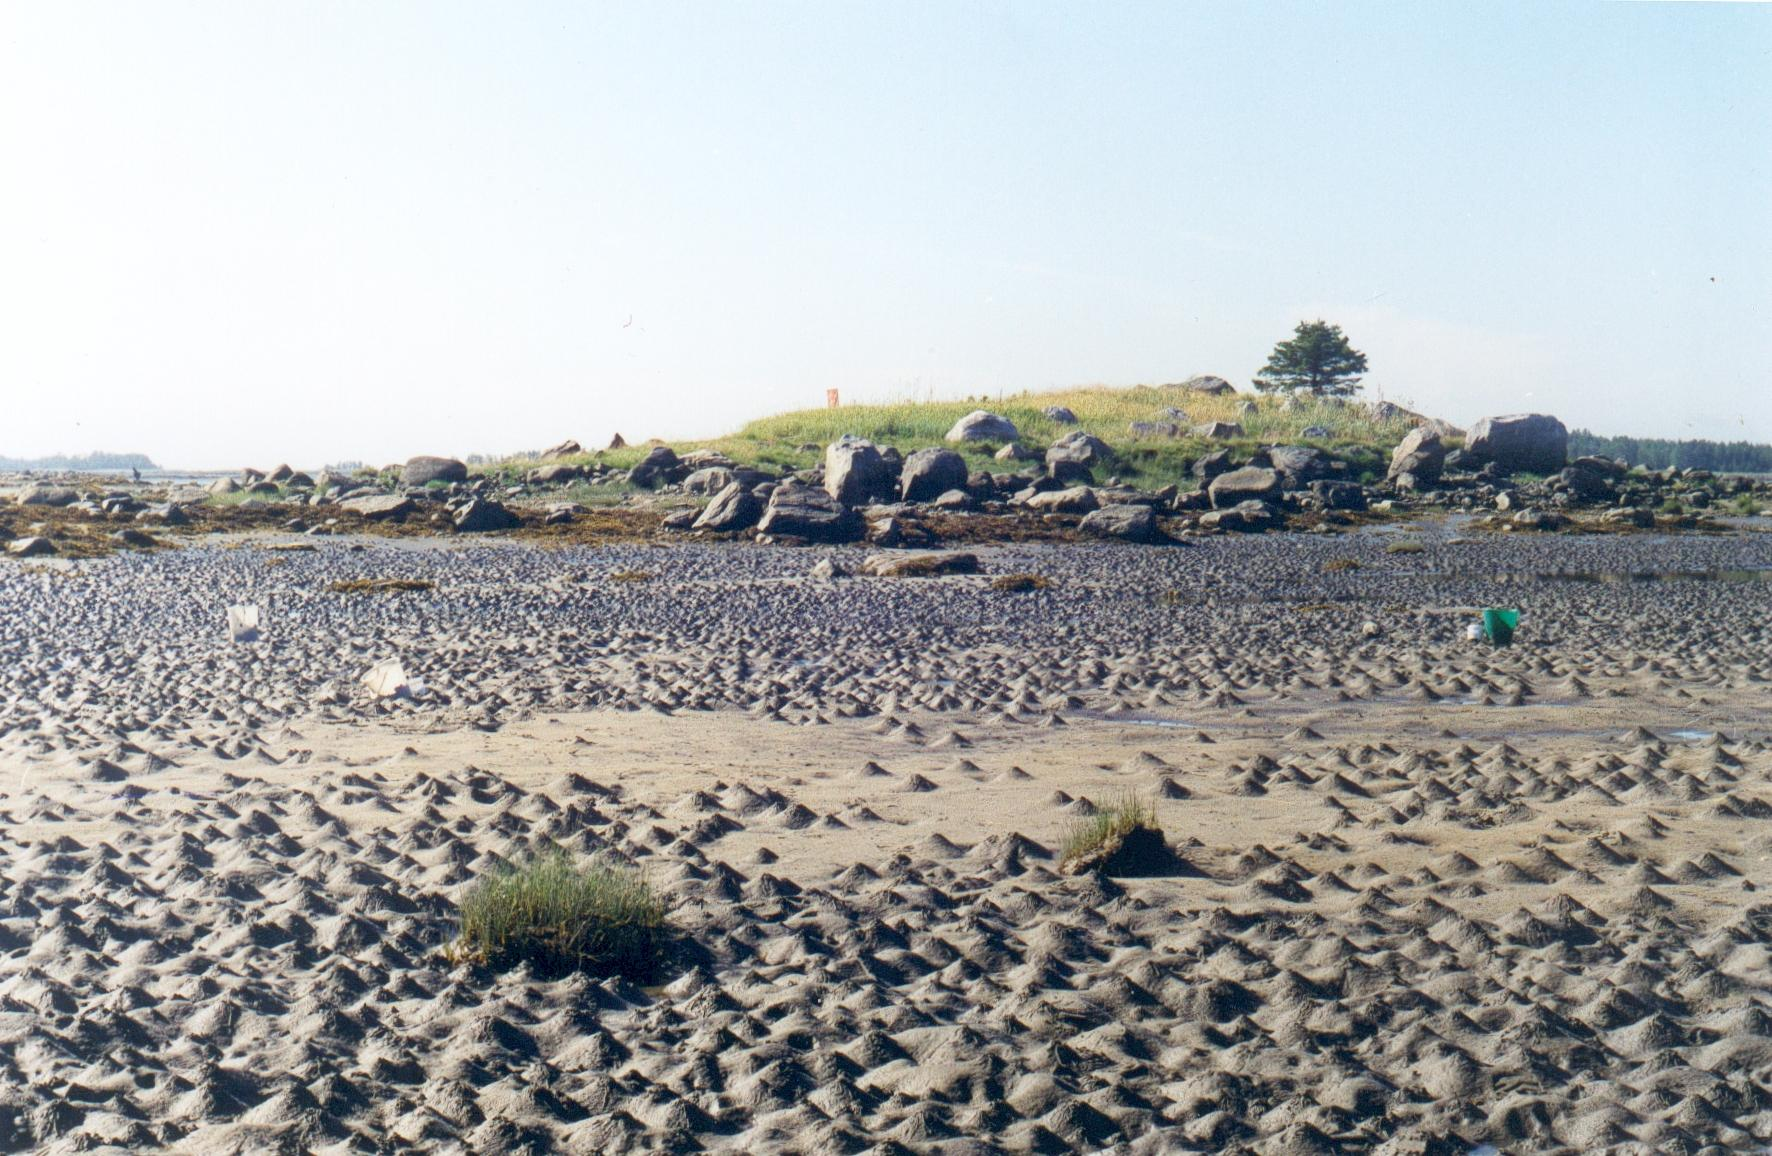
\includegraphics[height=.3\textheight]{Luvenga_Estuary.JPG}	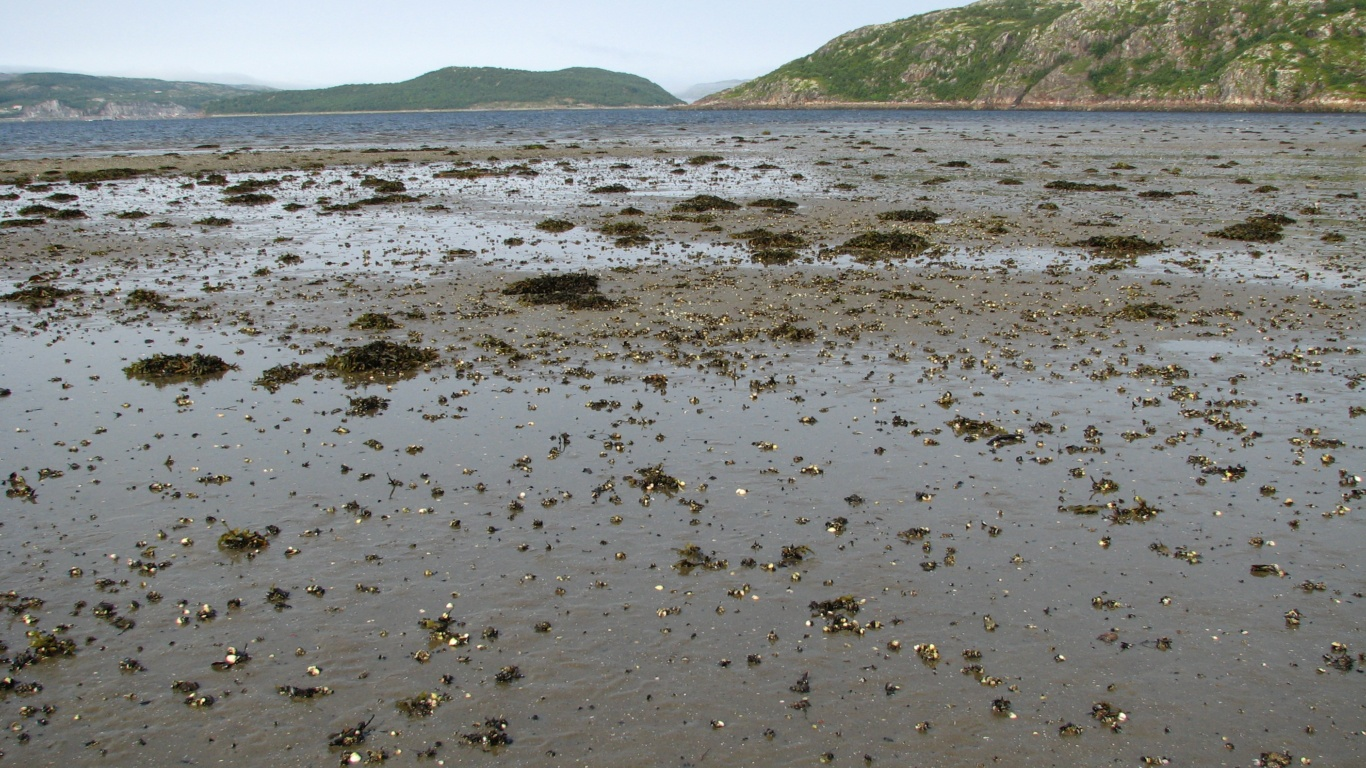
\includegraphics[height=.3\textheight]{Ura.JPG} 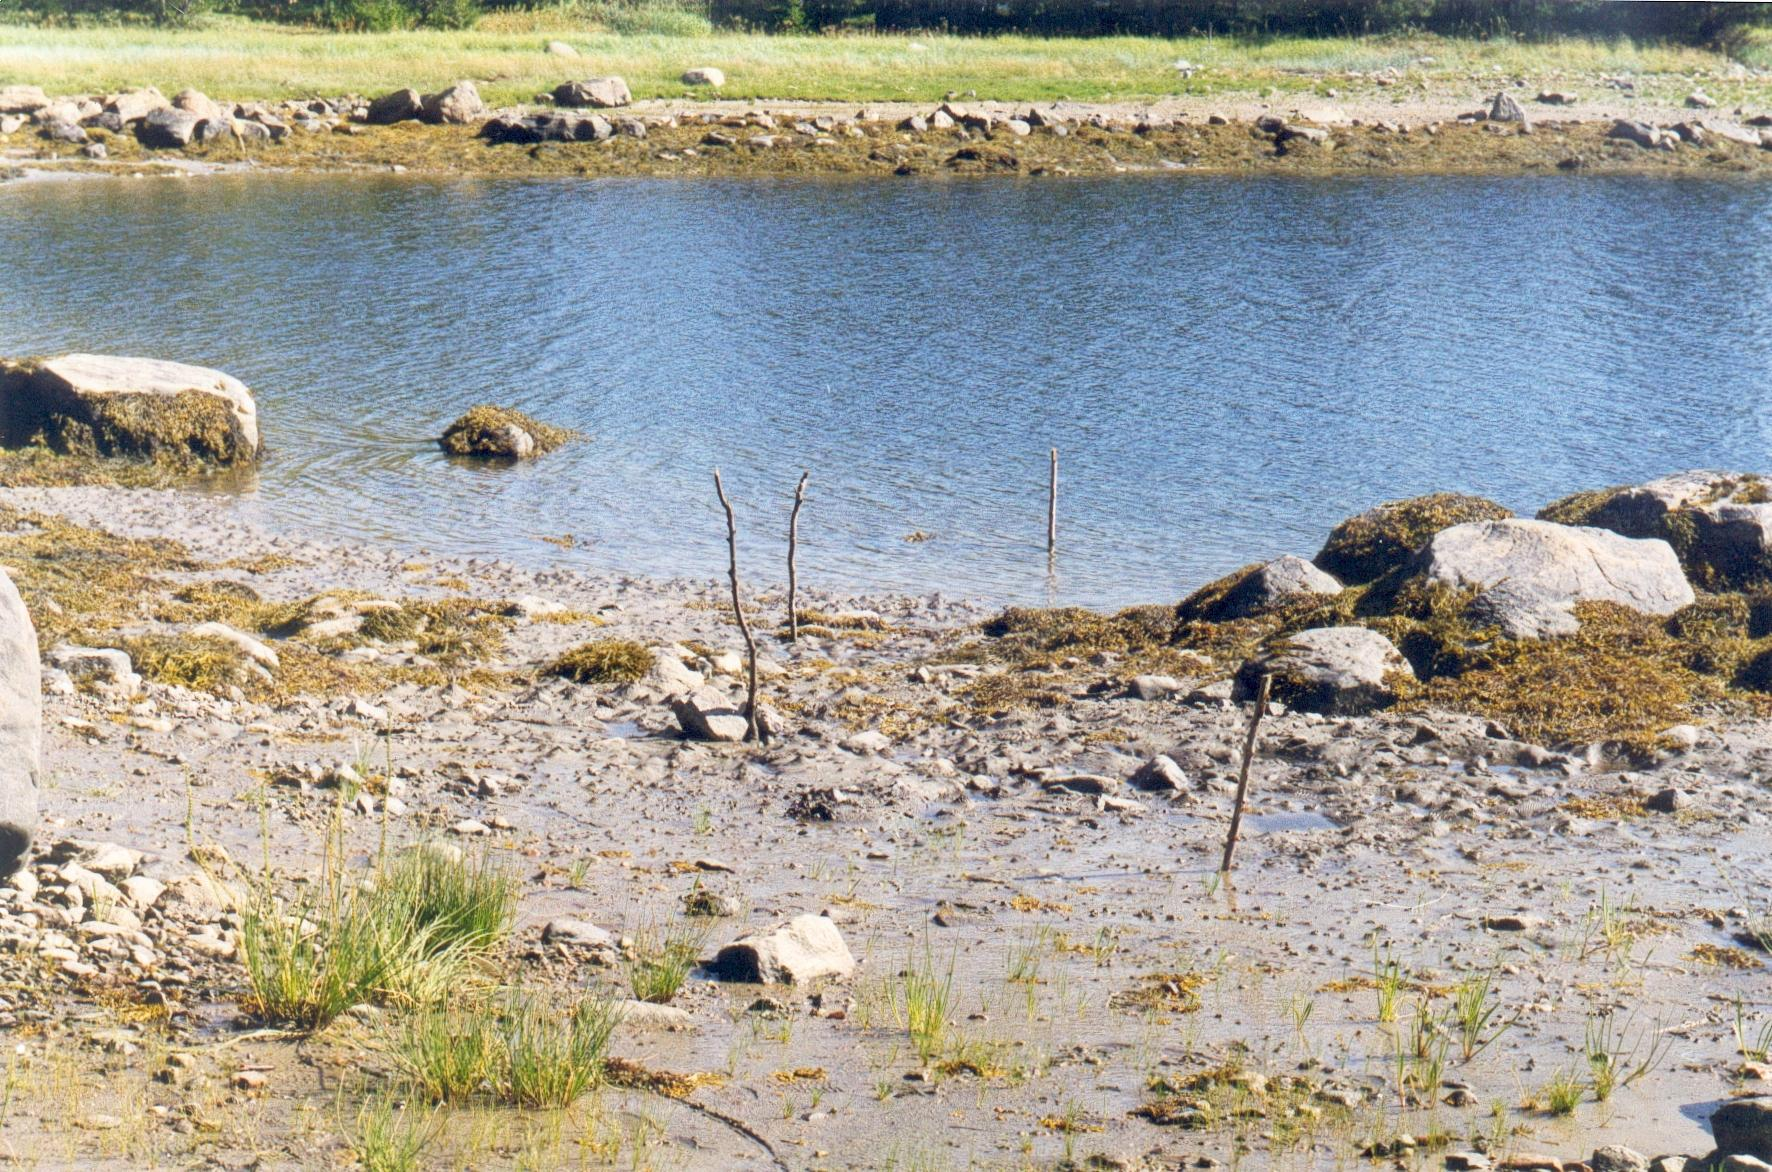
\includegraphics[height=.3\textheight]{Goreliy.JPG} %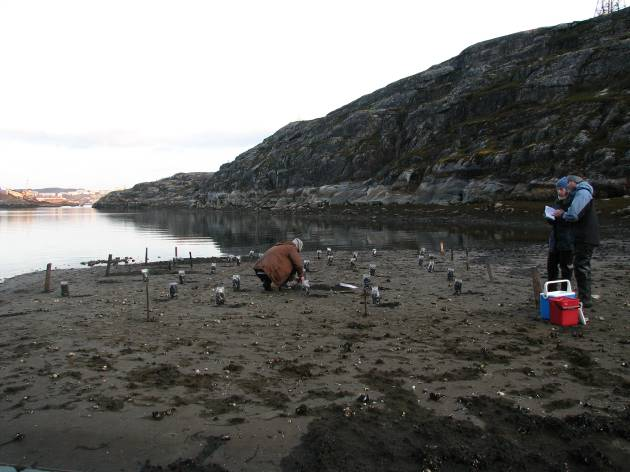
\includegraphics[height=.3\textheight]{Pala.JPG}


\end{frame}

\begin{frame}{\insertpagenumber.\ Цели и задачи}
\begin{description}
	\item[Цель.] Изучение организации поселений {\it Macoma balthica} в условиях осушной зоны Белого и Баренцева морей.

	\item[Задачи.]
Для этого были изучены следующие стороны организации поселений:
  \begin{enumerate}
    \item биотический и абиотический фон биотопов;
    \item структурные характеристики поселений \textit{M.~balthica} (показатели обилия, размерная структура);
    \item многолетняя динамика поселений \textit{M.~balthica};
    \item скорость линейного роста моллюсков;
    \item режим формирования спата.
  \end{enumerate}
\end{description}
\end{frame}


\begin{frame}{\insertpagenumber.\ Положения, выносимые на защиту}
\begin{scriptsize}

\begin{enumerate}
\item На литорали Кандалакшского залива Белого моря и в Баренцевом море (Западный Мурман и Кольский залив) \textit{Macoma balthica} формирует поселения, в которых плотность значительно варьирует во времени и может достигать нескольких тысяч экз./м$^2$, но наиболее типичны поселения маком с плотностью в несколько сотен экз./м$^2$. На литорали Восточного Мурмана Баренцева моря вид не формирует плотных поселений, и значения данного показателя редко превышает 100~экз./м$^2$.

\item Организация поселений  \textit{Macoma balthica} в условиях осушной зоны Белого и Баренцева морей не имеет принципиальных различий:
	\begin{itemize}
	\begin{scriptsize}
		\item  в типичном случае в многолетней динамике поселений сменяются мономодальный (преобладание молоди) и бимодальной (добавление второго модального класса~--- группы особей старшего возраста) типы размерной структуры; 
		\item как относительно редкое событие наблюдаются мономодальная структура поселений с ежегодным преобладаем молоди.
	\end{scriptsize}
	\end{itemize}

\item Характер динамики плотности поселений \textit{Macoma balthica} определяется, в основном, неравномерностью  уровня ежегодного пополнения их молодью. 
Беломорские поселения демонстрируют элементы синхронности процессов пополнения, что связано с влиянием температуры на выживаемость маком в первый год жизни  (численность однолетних особей после холодных зим с устойчивым ледоставом оказывается относительно выше) и спецификой условий в локальном местообитании.

\item Скорость роста особей \textit{Macoma balthica} в Белом и Баренцевом морях достоверно ниже, чем в других акваториях европейской части ареала вида. 
По характеру вариации средней скорости роста маком поселения Баренцева моря и Белого моря различий не имеют. 
\end{enumerate}
\end{scriptsize}
%\end{tiny}
\end{frame}


%%%%%%%%%%%%%%%%%%%%%%%%%%%%%%%%%%%%%%%%%%%%%%%%%%%%%
		\section[Методы]{Материал и методика}
%%%%%%%%%%%%%%%%%%%%%%%%%%%%%%%%%%%%%%%%%%%%%%%%%%%%%
\begin{frame}{\insertpagenumber.\ География исследований}
 \begin{center}
	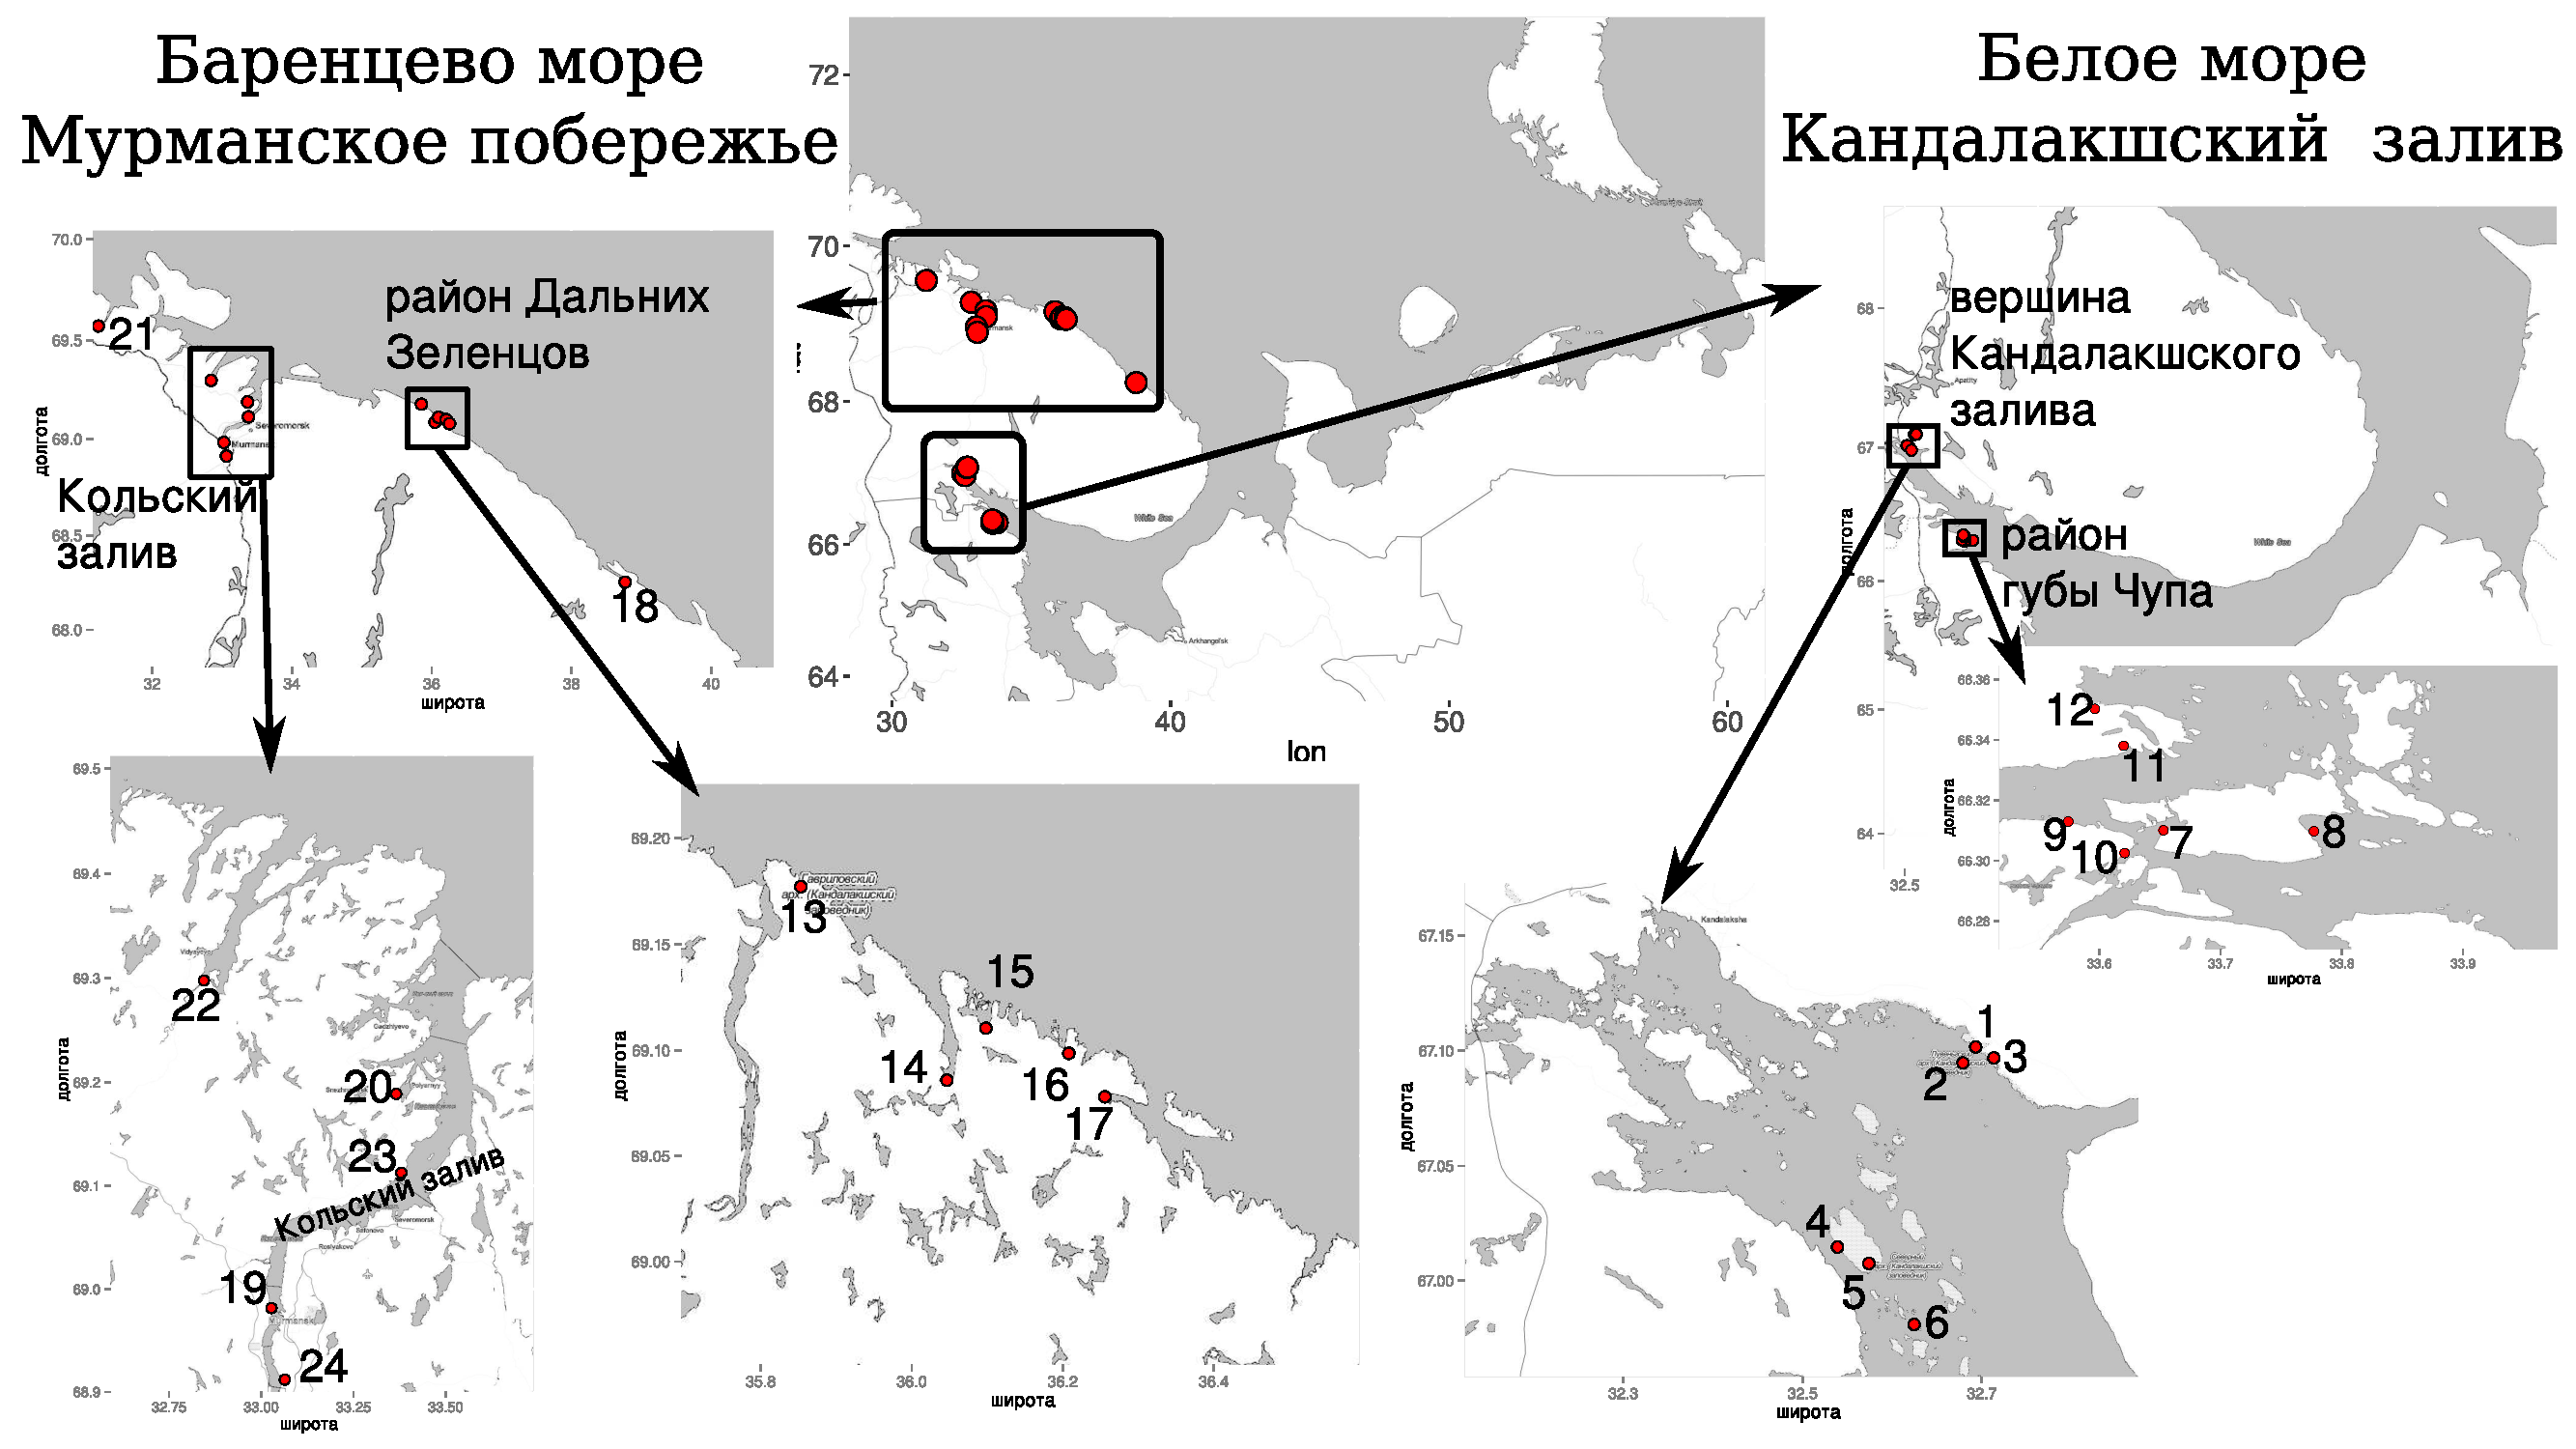
\includegraphics[height=.8\textheight]{./map_White_Barents.pdf}
 \end{center}
\end{frame}

\begin{frame}{\insertpagenumber.\ Материалы}
	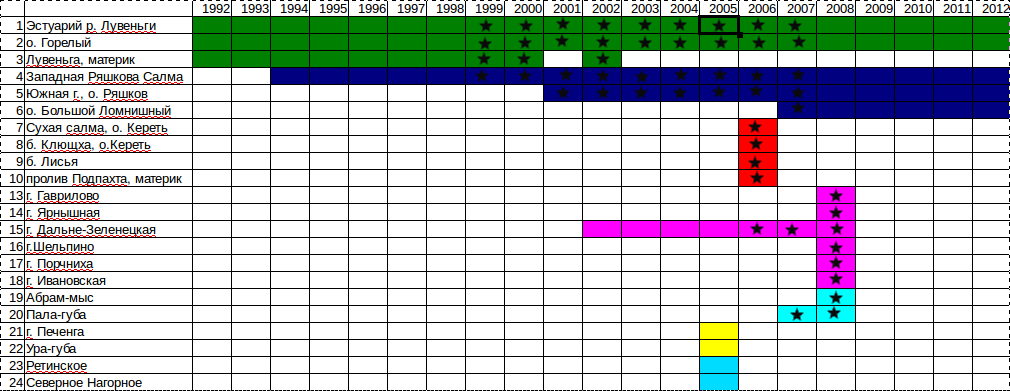
\includegraphics[width=\textwidth]{./timeline_field.png}

{\tiny Полевые сборы с участием автора отмечены звездой.\\
Цветовые обозначения районов: Красный~--- Керетский архипелаг, синий~--- Северный архипелаг, зеленый~--- Лувеньгские шхеры, голубой~--- Кольский залив, фиолетовый~--- Восточный Мурман}
\end{frame}

\begin{frame}{\insertpagenumber.\ Методы}
 \begin{center}
	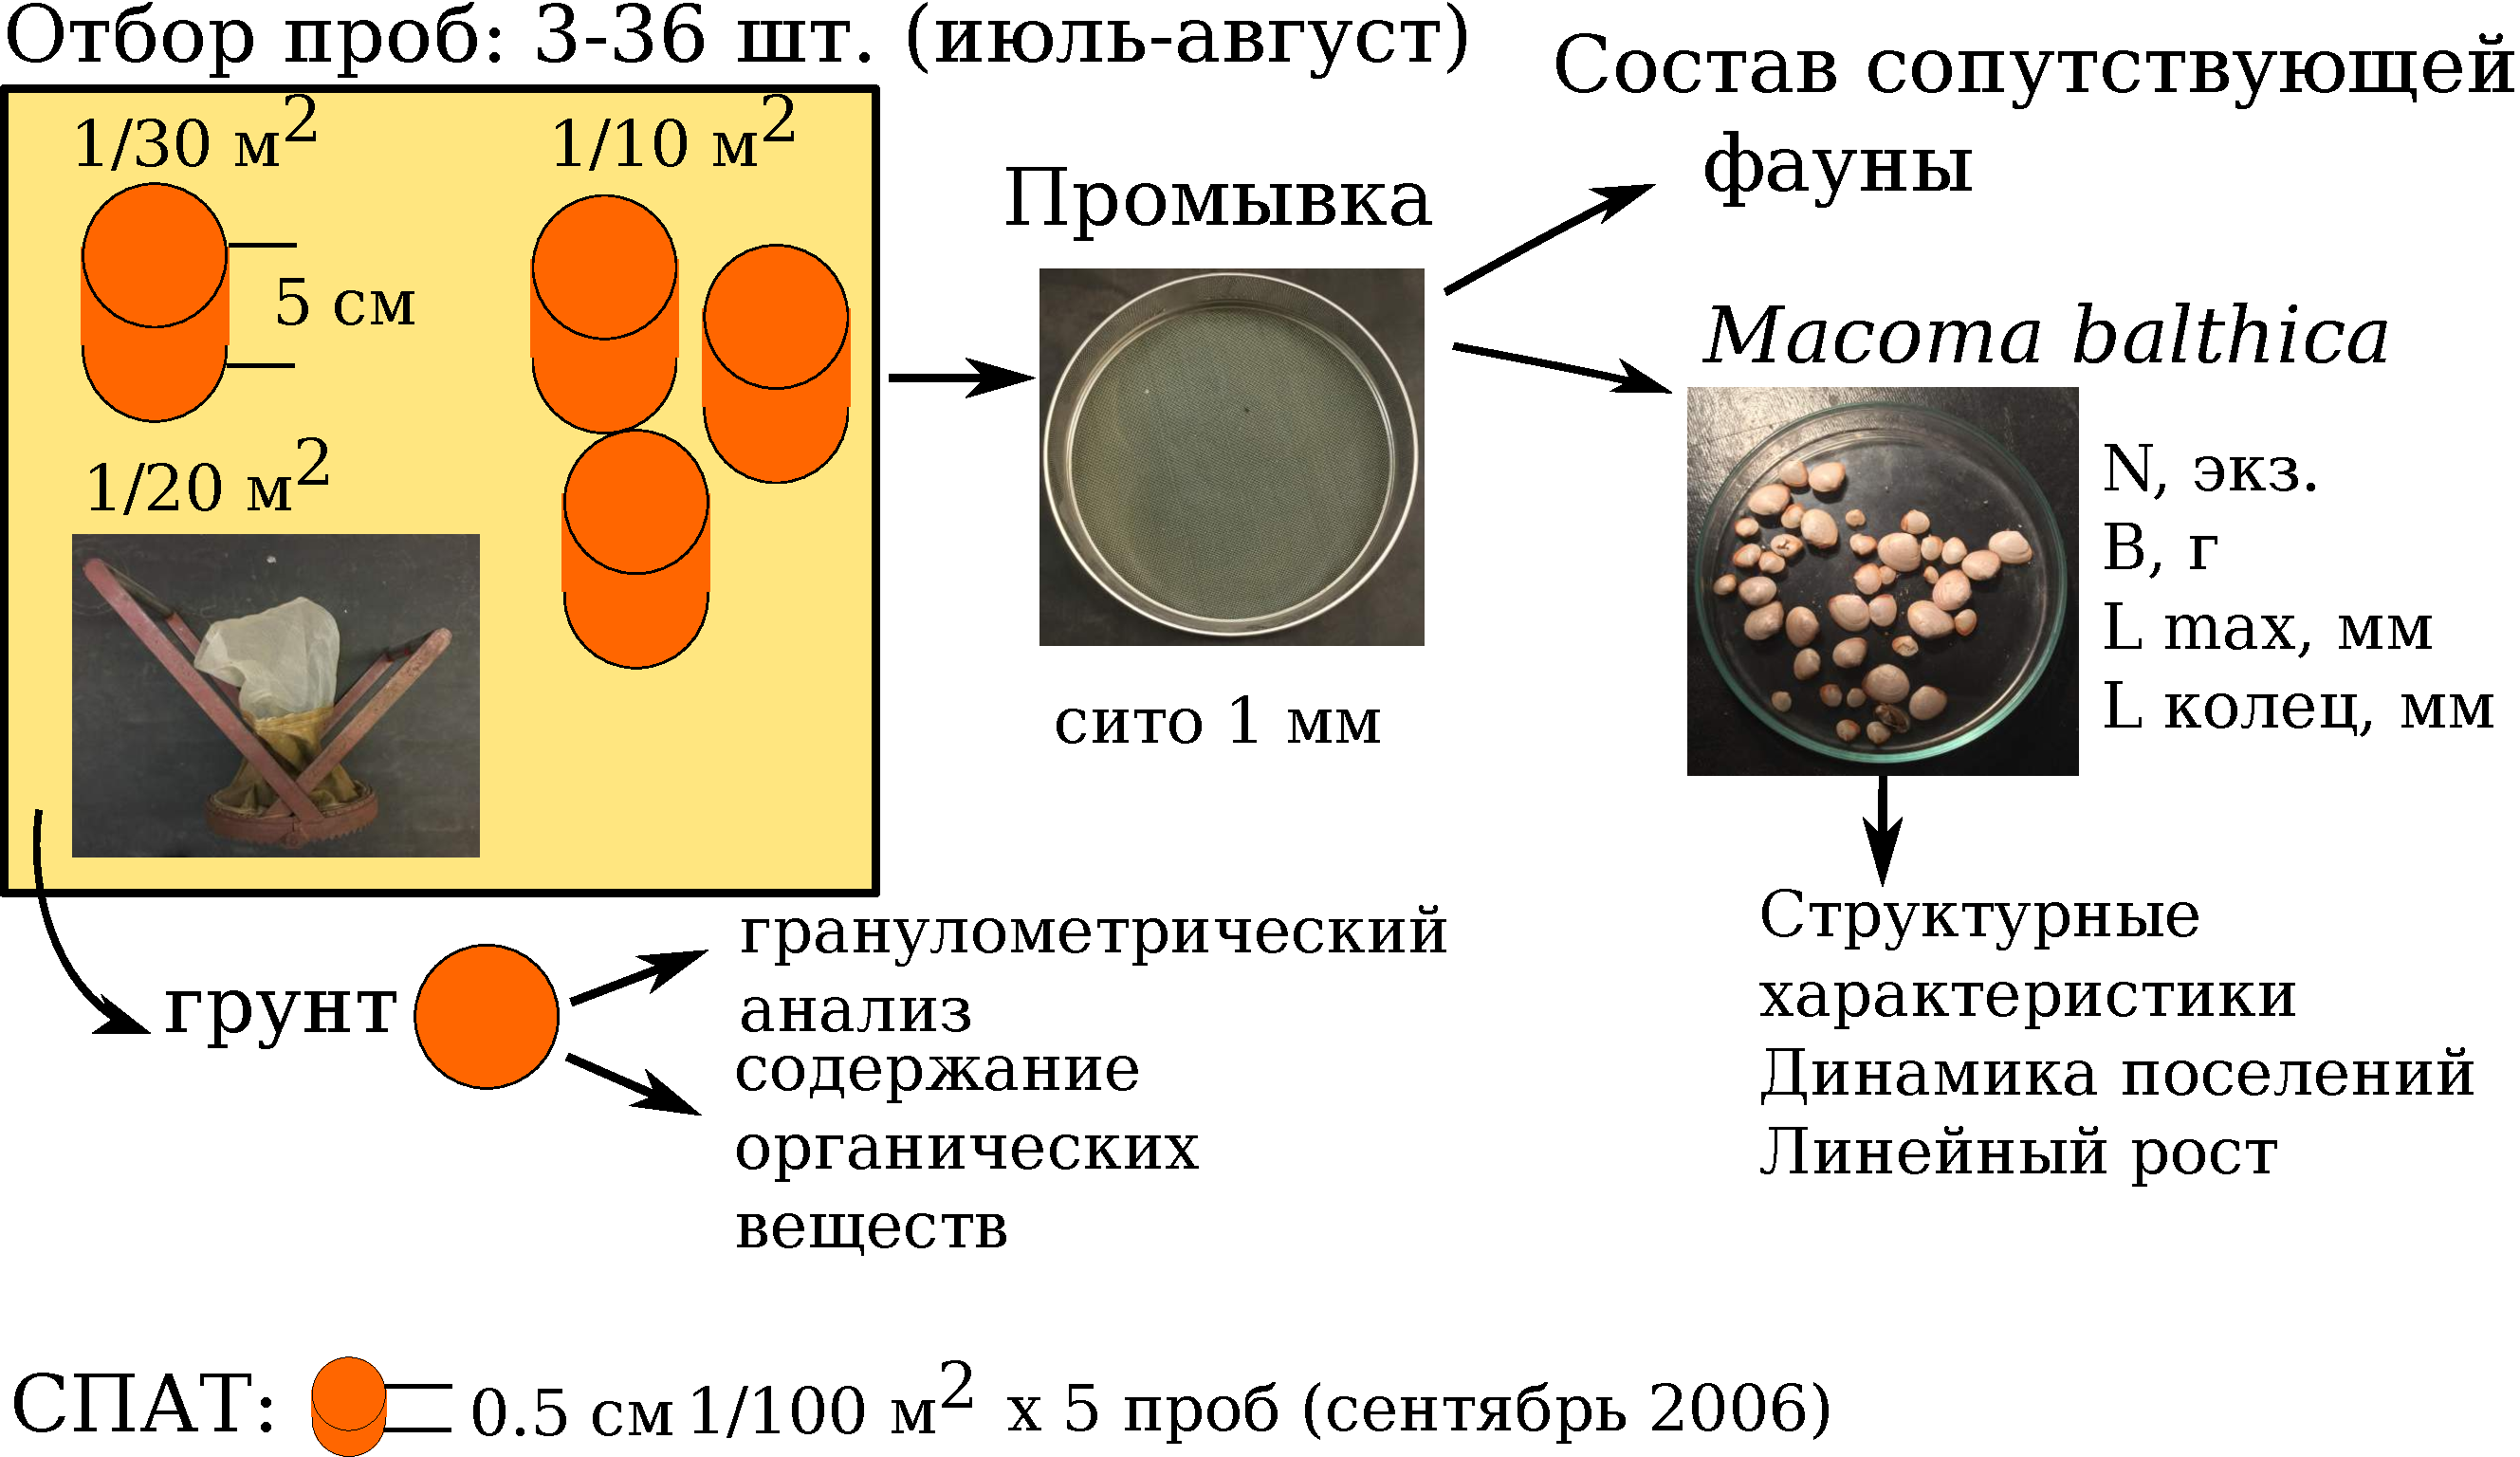
\includegraphics[height=.8\textheight]{./sampling_compressed.pdf}
 \end{center}
\end{frame}

%%%%%%%%%%%%%%%%%%%%%%%%%%%%%%%%%%%%%%%%%%%%%%%%%%%%%
		\section[Биотопы]{Биотический и абиотический фон биотопов}
%%%%%%%%%%%%%%%%%%%%%%%%%%%%%%%%%%%%%%%%%%%%%%%%%%%%%
\begin{frame}{\insertpagenumber.\ Условия обитания \textit{Macoma balthica} в Белом и Баренцевом морях}
\begin{scriptsize}
%\begin{small}
\begin{tabularx}{\textwidth}{|p{0.2\textwidth}|X|XX|} \hline
		& Белое море		    & \multicolumn{2}{c|}{Баренцево море:} \\
показатель	&	Кан\-да\-лакш\-ский залив &	Мурманское побережье & Кольский залив	\\ \hline \hline
\multicolumn{4}{|c|}{ТЕМПЕРАТУРА ВОДЫ:} \\ \hline 
min, $^{\circ}C$	&	{\large -0.5}	&	\multicolumn{2}{c|}{{\large3 -- 5}}  	\\
max, $^{\circ}C$	&	{\large15 (до 20)}	&	\multicolumn{2}{c|}{{\large8 (до 18)}}		\\ \hline \hline
\multicolumn{4}{|c|}{ГИДРОЛОГИЧЕСКАЯ СЕЗОННОСТЬ:} \\ \hline
макс. прогрев	& {\large лето}	&	\multicolumn{2}{c|}{{\large осень}}		\\
мин. прогрев	&	{\large зима}	&	\multicolumn{2}{c|}{{\large весна}}		\\ \hline \hline
\multicolumn{4}{|c|}{СОЛЕНОСТЬ:} \\ \hline
средне\-годовая, \permil &	{\large 23 -- 25}	&	{\large 34}	&	{\large 28}	\\
min, \permil &	{\large 10}	&	{\large 28}	&	{\large 2}	 \\ \hline \hline
про\-дол\-жи\-тель\-ность ле\-дос\-тава, мес.	&	{\large 5 -- 6} 	& \multicolumn{2}{c|}{{\large 0}, припай в отдельных губах}		\\ \hline
%высота приливной волны, м	&	3	&	4		\\ \hline
\end{tabularx}
\end{scriptsize}
%\end{small}
{\tiny (По: Дерюгин, 1915; Гурьянова и др., 1928 -- 1920; Кузнецов, 1960; Бабков, Голиков, 1984; Berger et al., 2003; \textit{Кольский меридиан, 2014})}
\end{frame}


%\begin{frame}{\insertpagenumber.\ Термические характеристики исследованных акваторий}

%{\scriptsize (По: Berger et al., 2003; \textit{Кольский меридиан, 2014})}
%		\begin{center}
%			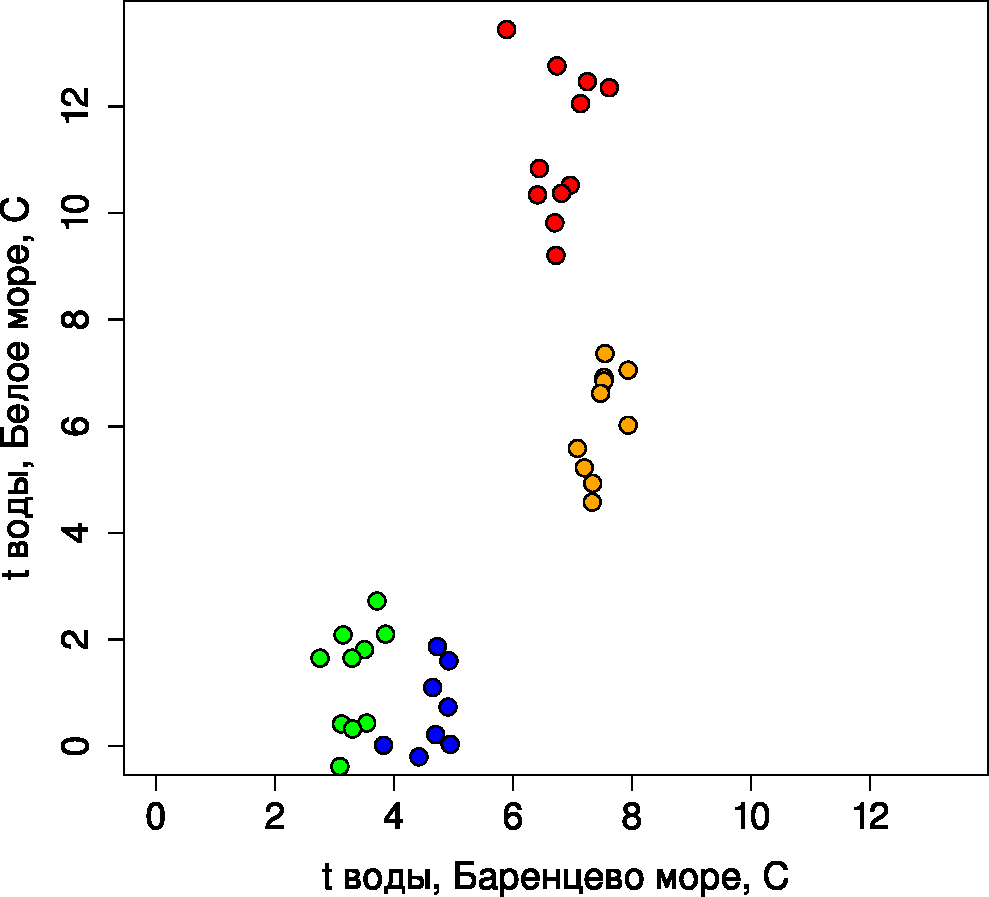
\includegraphics[height=0.8\textheight]{temp_White_Barents_big1.pdf}
%		\end{center}
%{\scriptsize Цветовые обозначения: синий~--- зима, зеленый~--- весна, красный~--- лето, желтый~--- осень}
%\end{frame}


\begin{frame}{\insertpagenumber.\ Гранулометрический состав грунта в исследованных биотопах}

			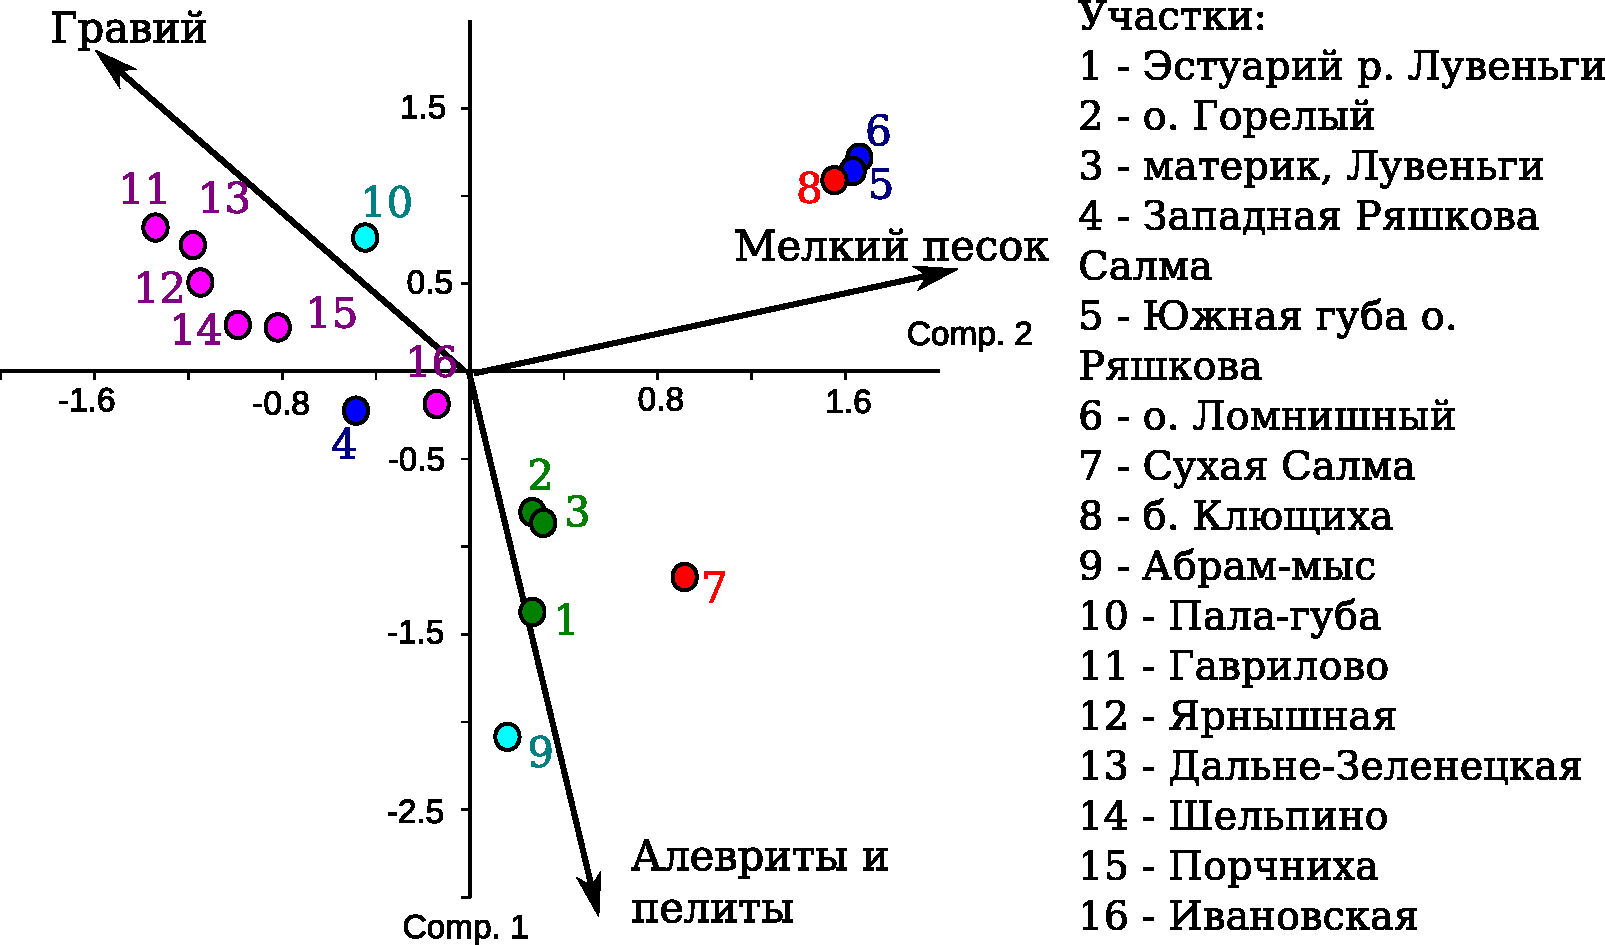
\includegraphics[width=.75\textwidth]{pca_grunt.pdf}

{\tiny Анализ главных компонент массовых долей фракций грунта с различным диаметром частиц}
%	\begin{minipage}[t]{.49\linewidth}
%		\begin{center}
%		{\footnotesize Белое море}
%			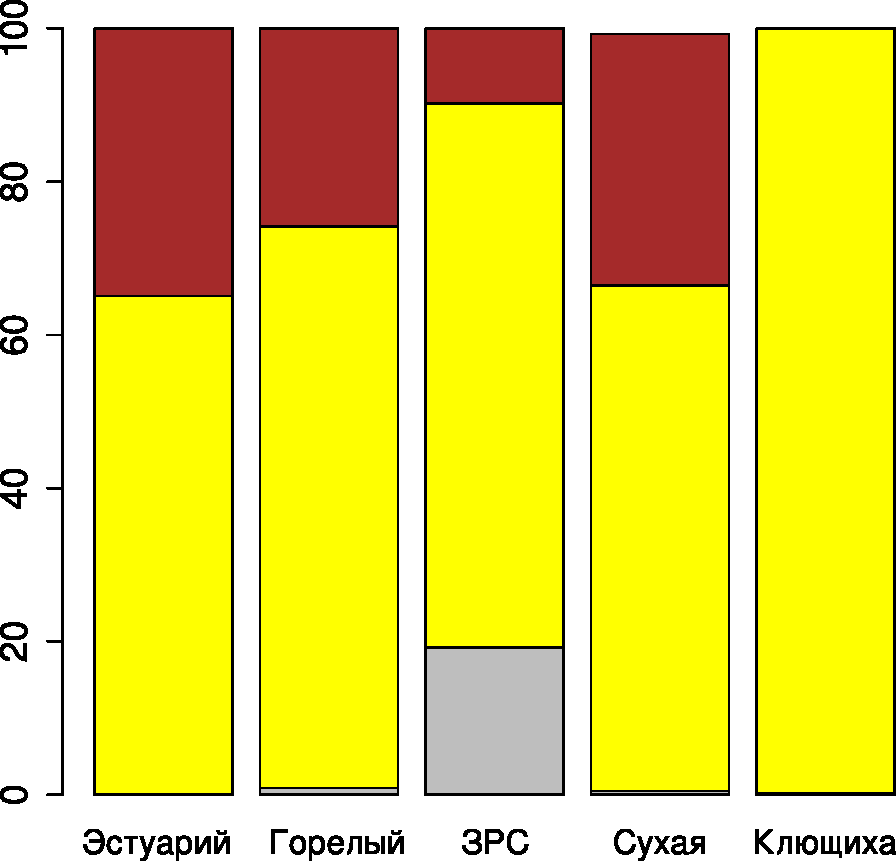
\includegraphics[width=\textwidth]{grunty_white1.pdf}
%		\end{center}
%	\end{minipage}
%
%	\begin{minipage}[t]{.49\linewidth}
%		\begin{center}
%		{\footnotesize Баренцево море}
%			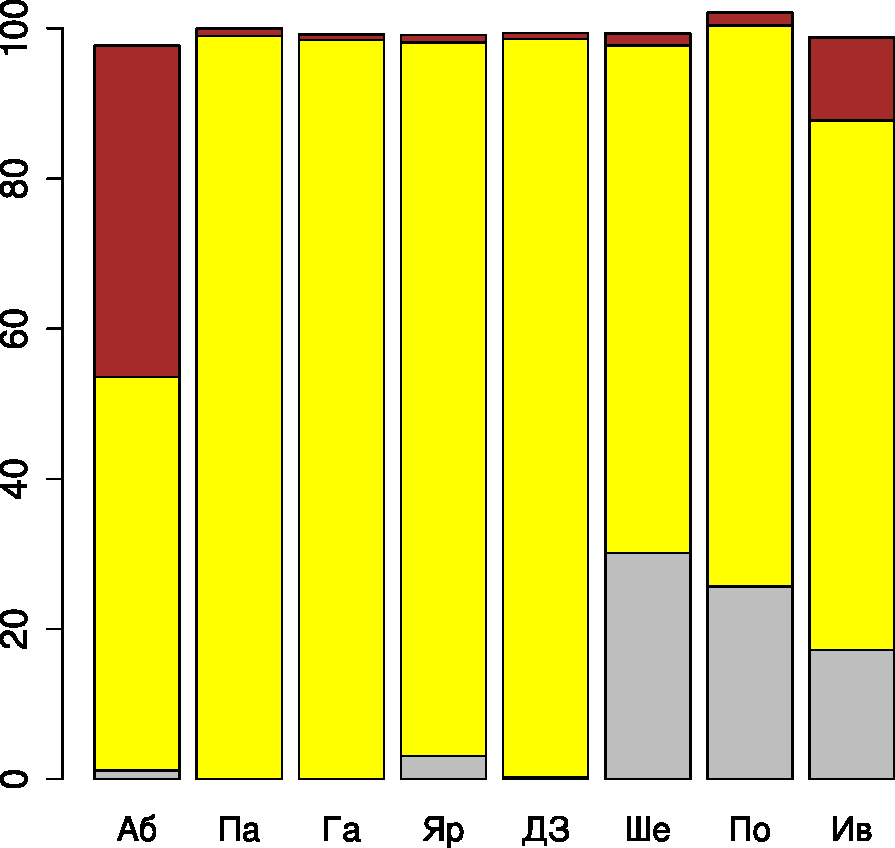
\includegraphics[width=\textwidth]{grunty_barents1.pdf}
%		\end{center}
%	\end{minipage}

%\begin{tiny} 
%Обозначения участков: ЗРС~--- Западная Ряшкова Салма, Аб~--- Абрам-мыс, Па~--- Пала-губа, Га~--- Гаврилово, Яр~--- Ярнышная, ДЗ~--- Дальне-Зеленецкая, Ше~--- Шельпино, По~--- Порчниха, Ив~--- Ивановская.\\
%\end{tiny}
%{\scriptsize Цветовые обозначения: серый~--- гравий, желтый~--- песок, коричневый~--- алевриты и пелиты.}
{\tiny Цветовые обозначения районов: Красный~--- Керетский архипелаг, синий~--- Северный архипелаг, зеленый~--- Лувеньгские шхеры, голубой~--- Кольский залив, фиолетовый~--- Восточный Мурман}
\end{frame}

\begin{frame}{\insertpagenumber.\ Совокупное таксономическое разнообразие в сообщестах}
			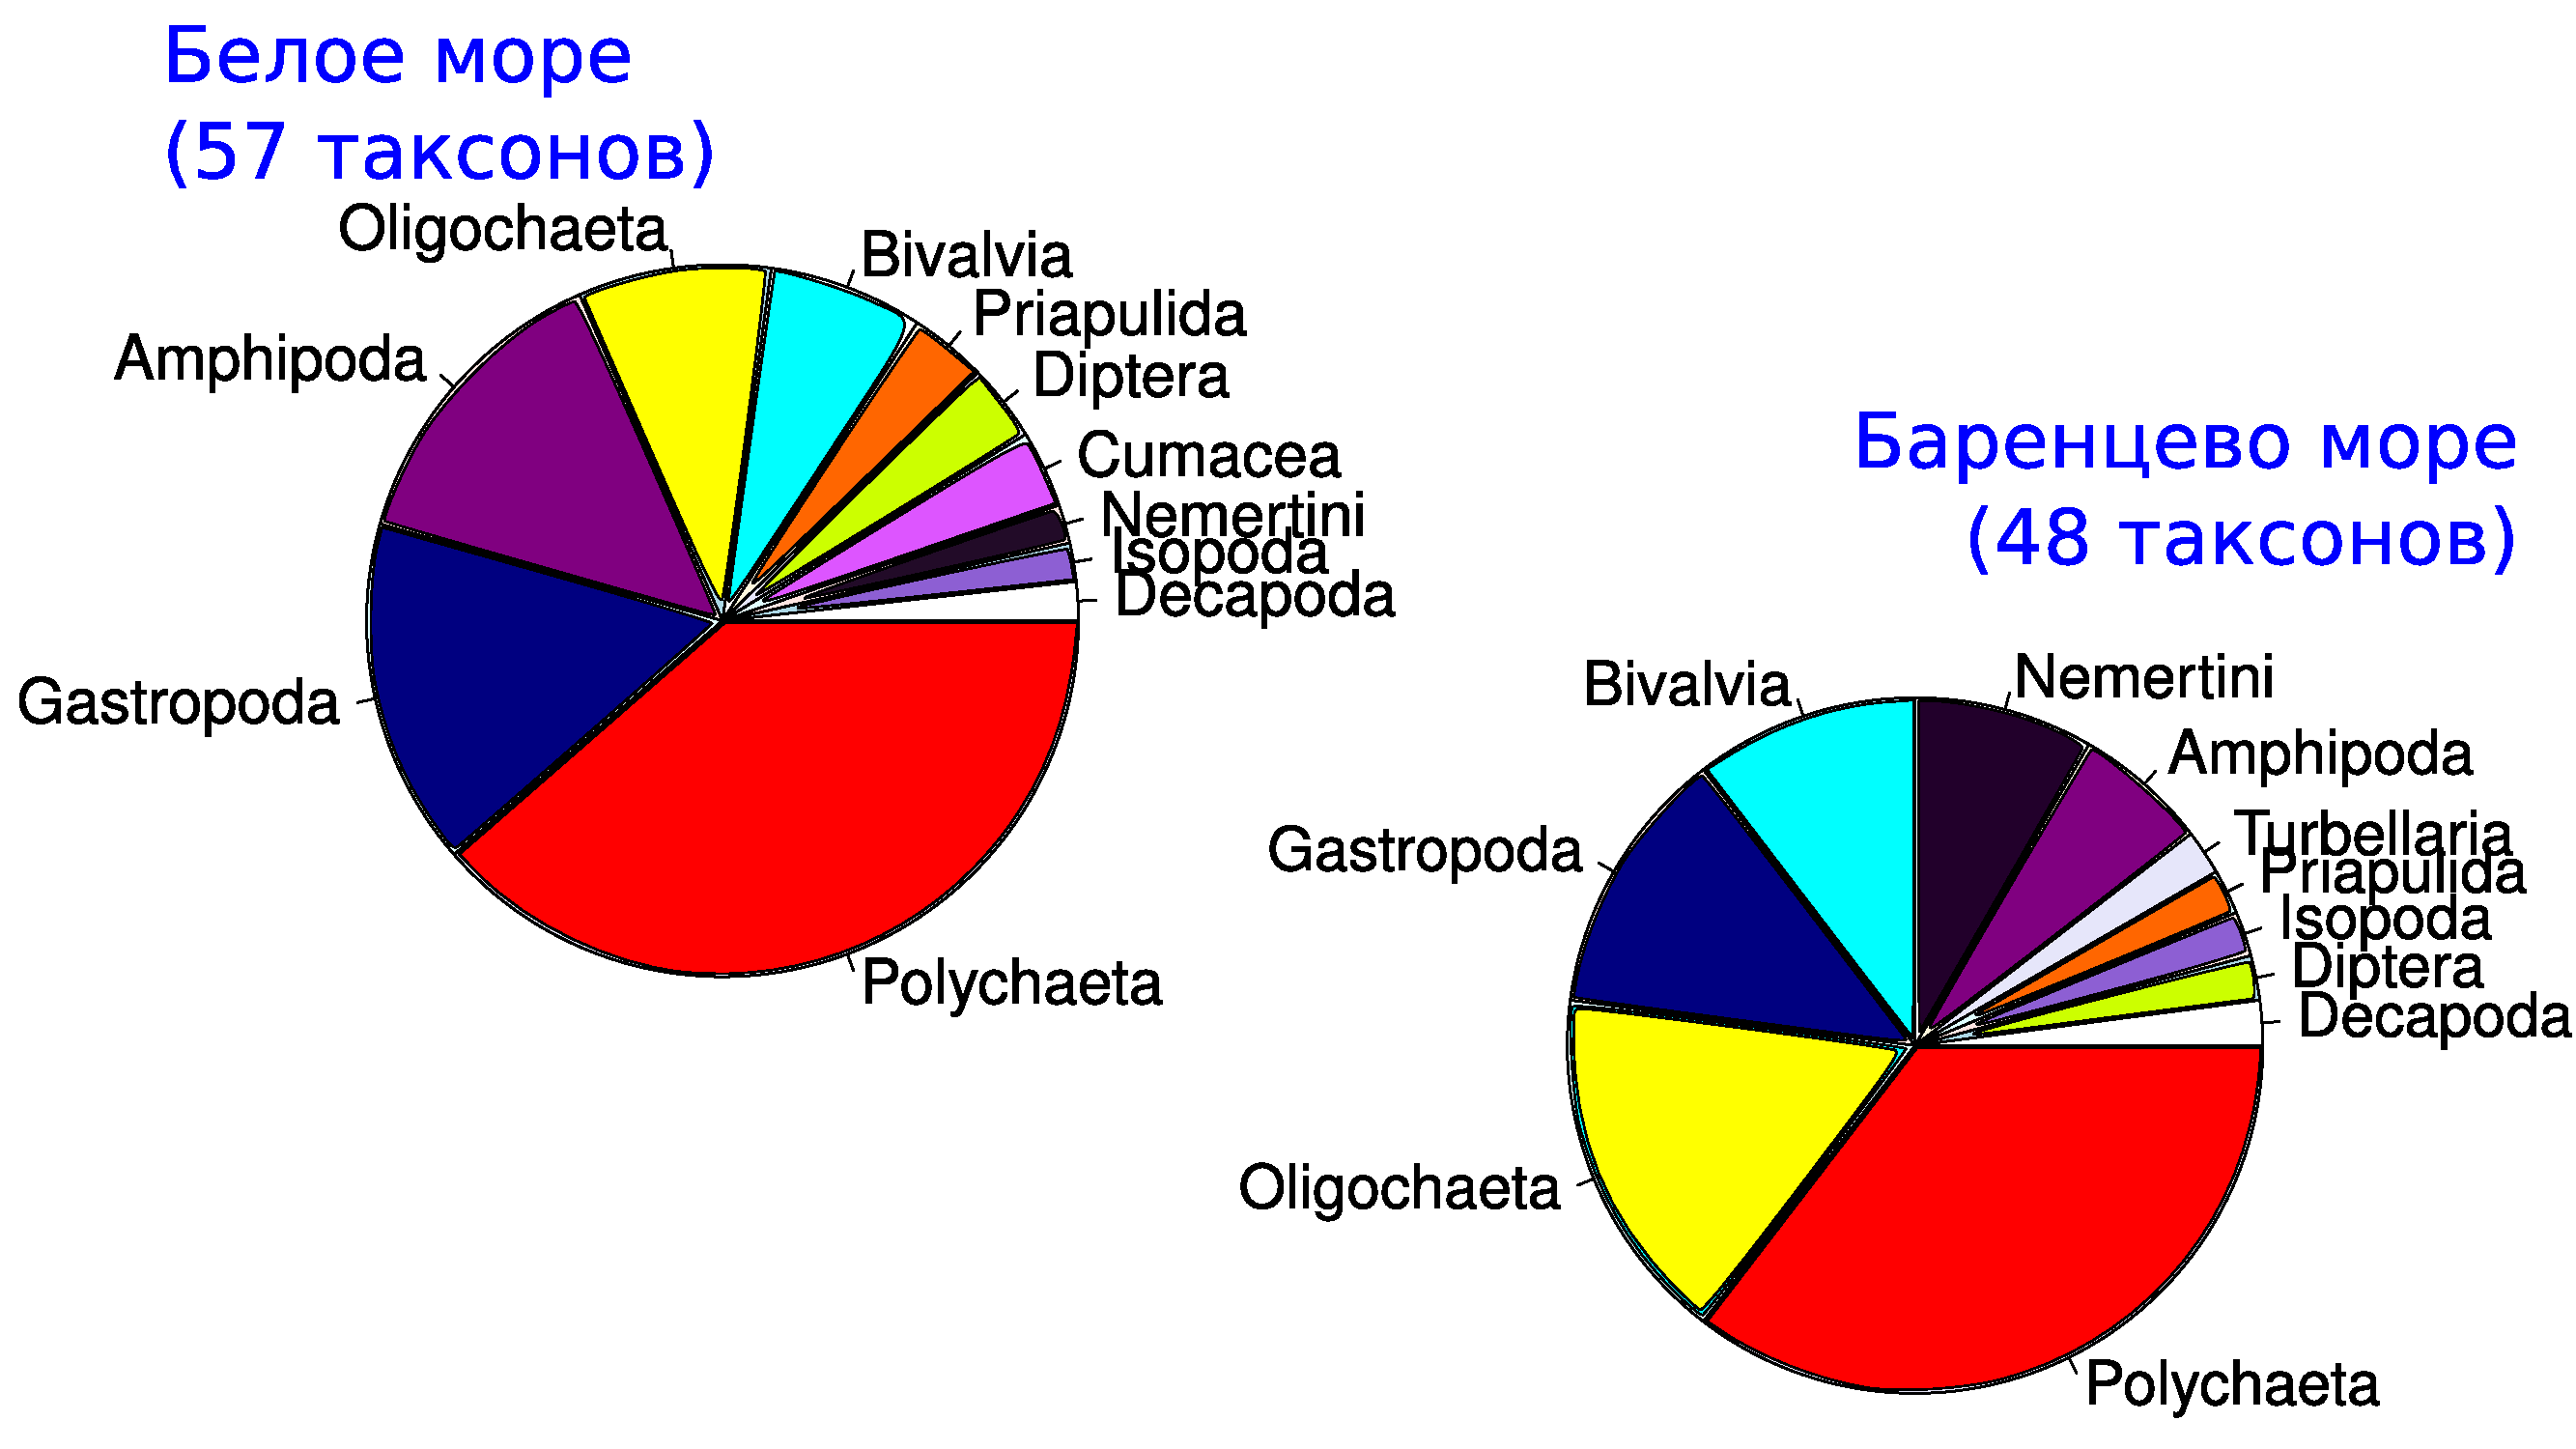
\includegraphics[width=\textwidth]{taxa.pdf}
\end{frame}


%%%%%%%%%%%%%%%%%%%%%%%%%%%%%%%%%%%%%%%%%%%%%%%%%%%%%
		\section[Обилие]{Обилие {\it Macoma balthica}}
%%%%%%%%%%%%%%%%%%%%%%%%%%%%%%%%%%%%%%%%%%%%%%%%%%%%%
\begin{frame}{\insertpagenumber.\ Обилие {\it M.~balthica} в Белом море}
	\begin{minipage}[t]{.49\linewidth}
		\begin{center}
		{\footnotesize Плотность поселения}
			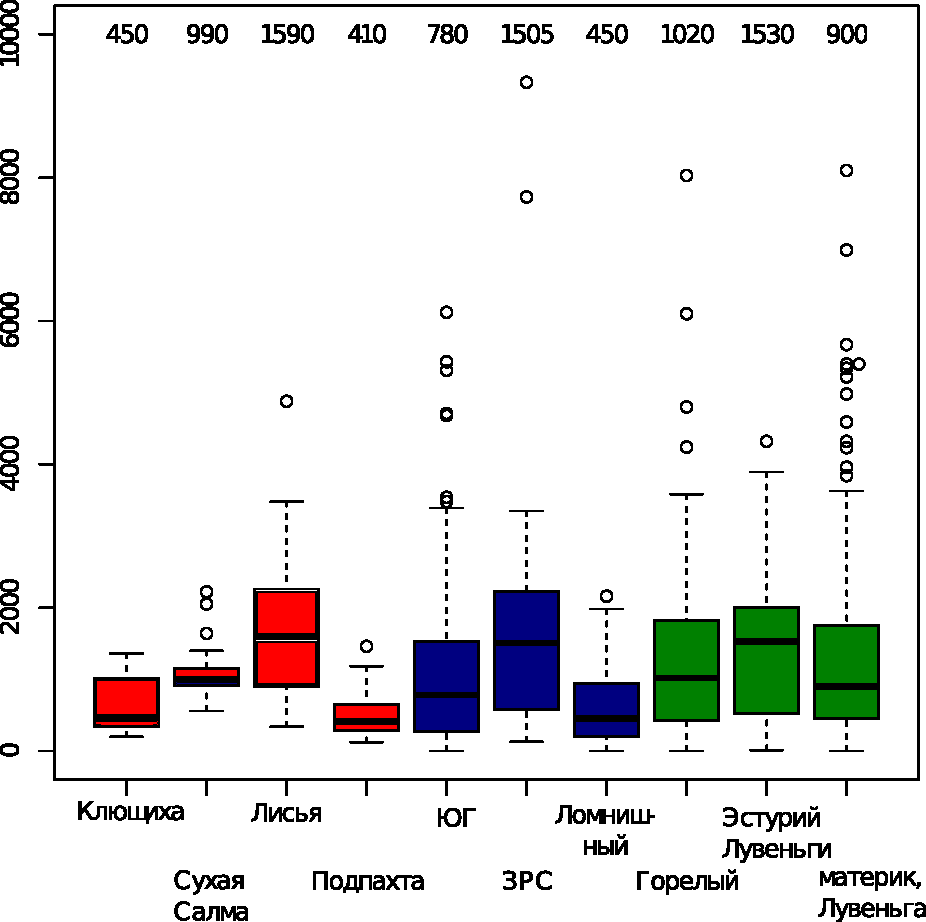
\includegraphics[width=.9\textwidth]{N2_area_White2.pdf}
		\end{center}
	\end{minipage}
%
	\begin{minipage}[t]{.49\linewidth}
		\begin{center}
		{\footnotesize Биомасса}
			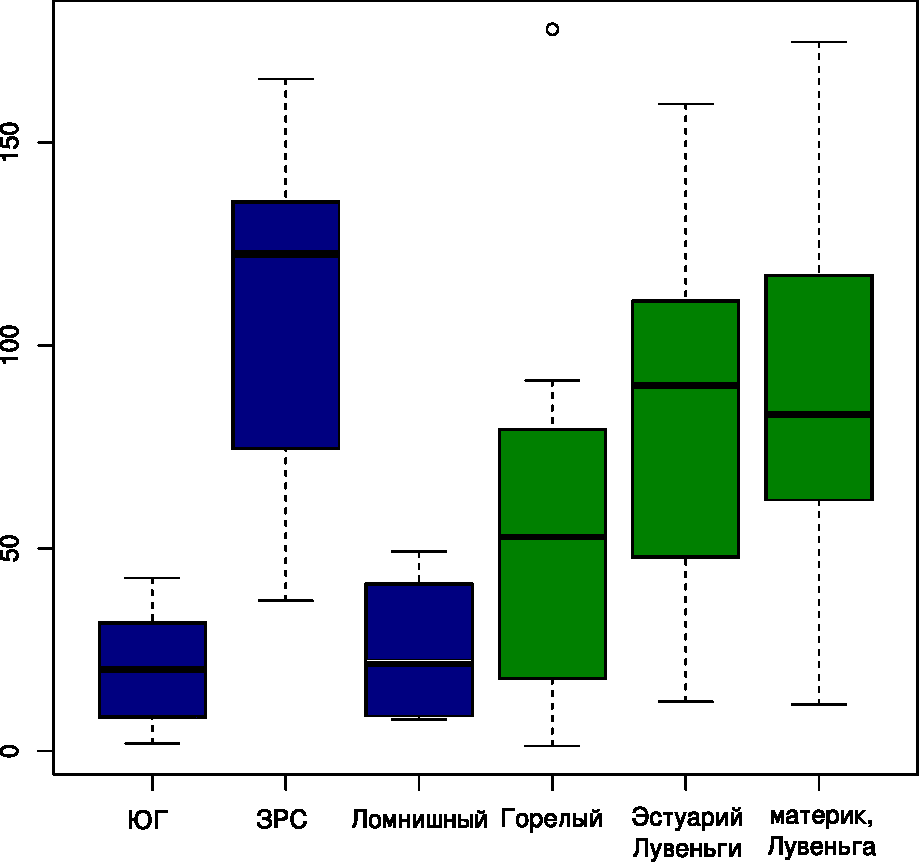
\includegraphics[width=.9\textwidth]{B_Kanda_ru2.pdf}
		\end{center}
	\end{minipage}


{\scriptsize Районы: Керетский арх.~--- красный, Северный арх.~--- синий, Лувеньгские шхеры~--- зеленый.}\\
\begin{tiny} 
Жирная горизонтальная линия~--- медианное значение показателя;
границы <<ящика>>~--- 1 и 3 квартили; <<усы>>~--- 1,5 интерквартильного расстояния;
точки~--- значения, выпадающие за 1,5 интерквартильных расстояния.
Числа в верхней части графика~--- средние значения плотности поселений маком, экз./м$^2$.
\end{tiny}

\end{frame}



\begin{frame}{\insertpagenumber.\ Обилие {\it M.~balthica} в Баренцевом море}
	\begin{minipage}[t]{.49\linewidth}
		\begin{center}
		{\footnotesize Плотность поселения}
			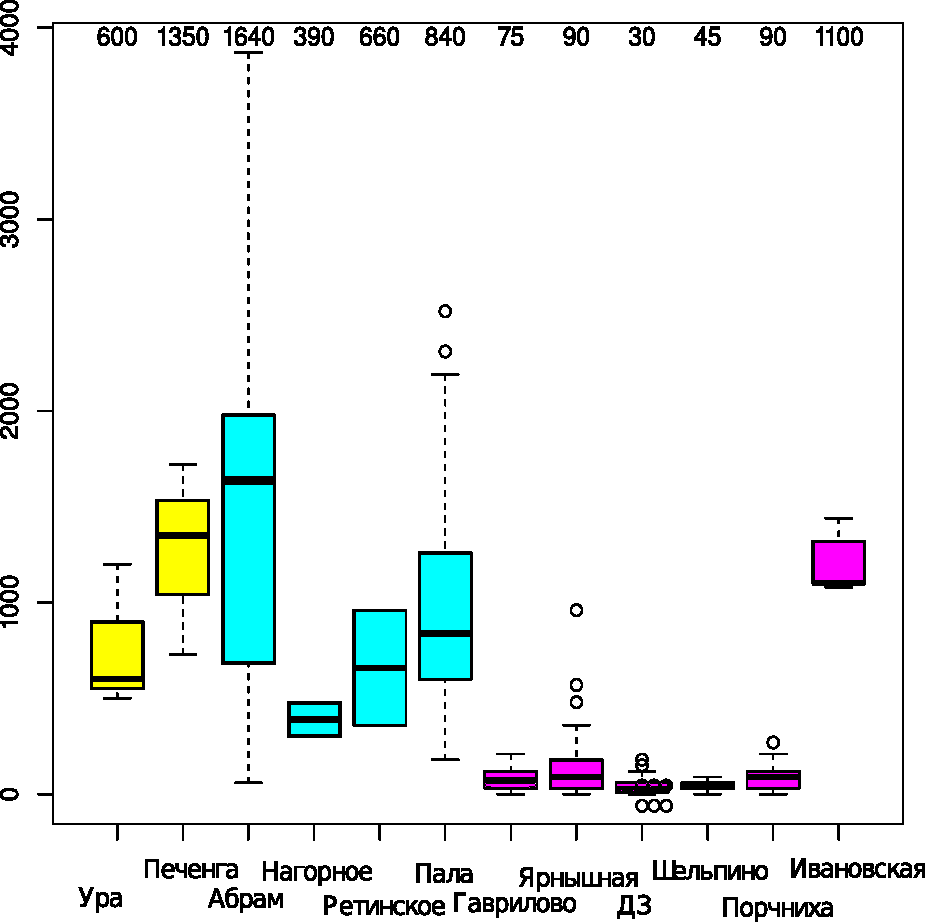
\includegraphics[width=.9\textwidth]{N2_area_Barents2.pdf}
		\end{center}
	\end{minipage}
%
	\begin{minipage}[t]{.49\linewidth}
		\begin{center}
		{\footnotesize Биомасса}
			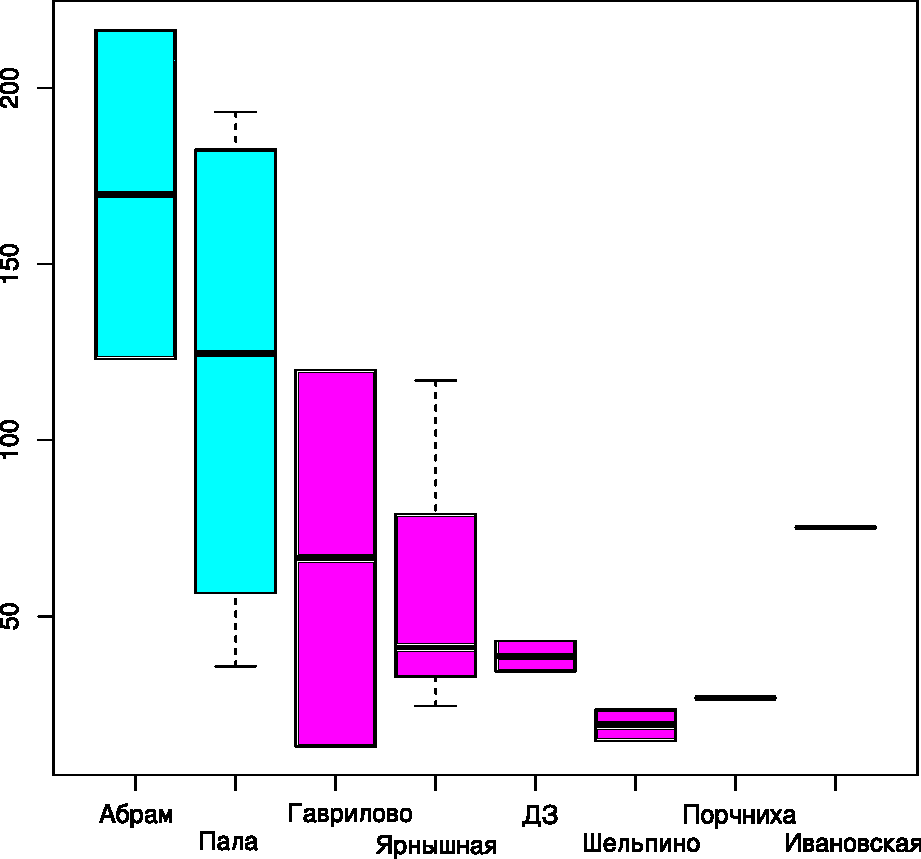
\includegraphics[width=.9\textwidth]{B_Barents_uchastki_ru2.pdf}
		\end{center}
	\end{minipage}


{\scriptsize Районы: Зап. Мурман~--- желтый, Кольский залив~--- голубой, Вост. Мурман~--- фиолетовый.}\\
\begin{tiny}
 Жирная горизонтальная линия~--- медианное значение показателя;
границы <<ящика>>~--- 1 и 3 квартили; <<усы>>~--- 1,5 интерквартильного расстояния;
точки~--- значения, выпадающие за 1,5 интерквартильных расстояния.
Числа в верхней части графика~--- средние значения плотности поселений маком, экз./м$^2$.
\end{tiny}
\end{frame}



\begin{frame}{\insertpagenumber.\ Обилие {\it M.~balthica} в европейской части ареала}
	\begin{minipage}[t]{.49\linewidth}
		\begin{center}
		{\footnotesize Плотность поселения}
			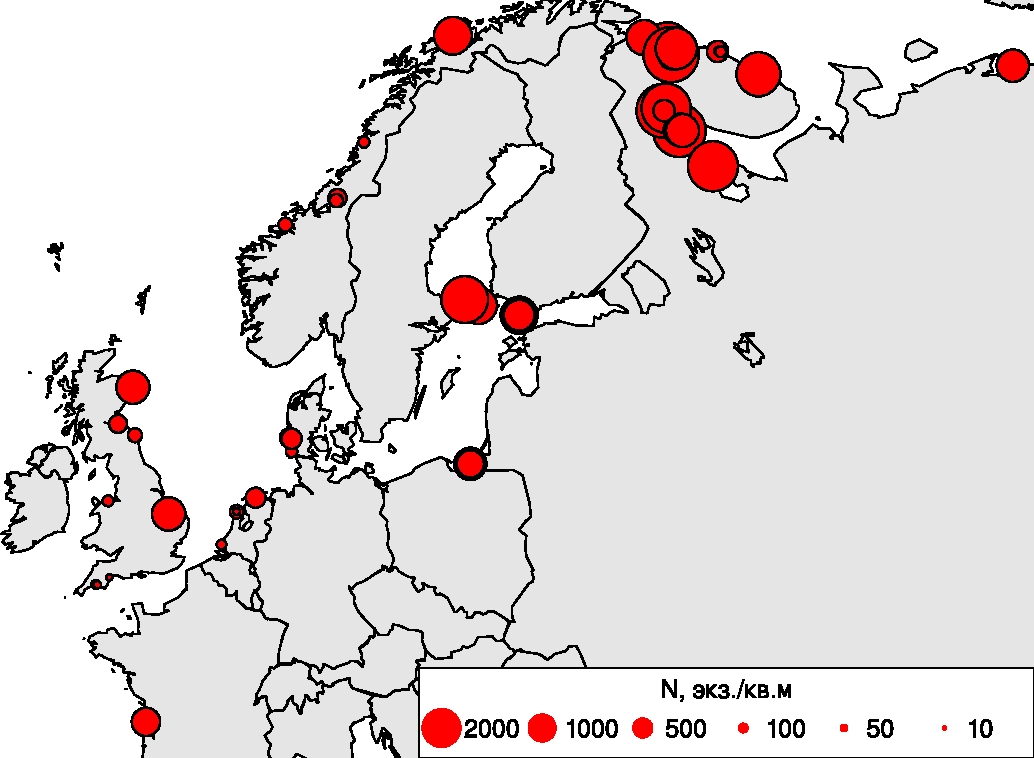
\includegraphics[width=.9\textwidth]{Nmean_ru1.pdf}\\[1ex]
			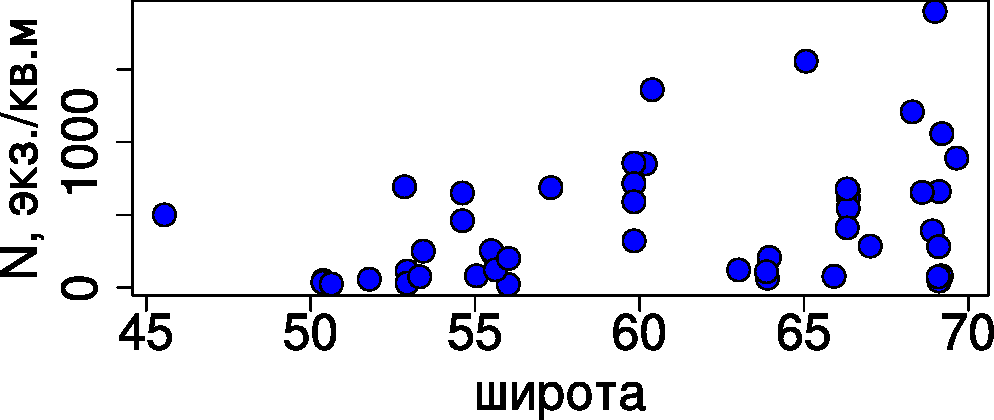
\includegraphics[width=.9\textwidth]{lat_vs_Nmean_big1.pdf}\\
{\scriptsize Корреляция Спирмена: $r_{s} = -0,43$, $p < 0,001$.}
		\end{center}
	\end{minipage}
%
	\begin{minipage}[t]{.49\linewidth}
		\begin{center}
		{\footnotesize Биомасса}
			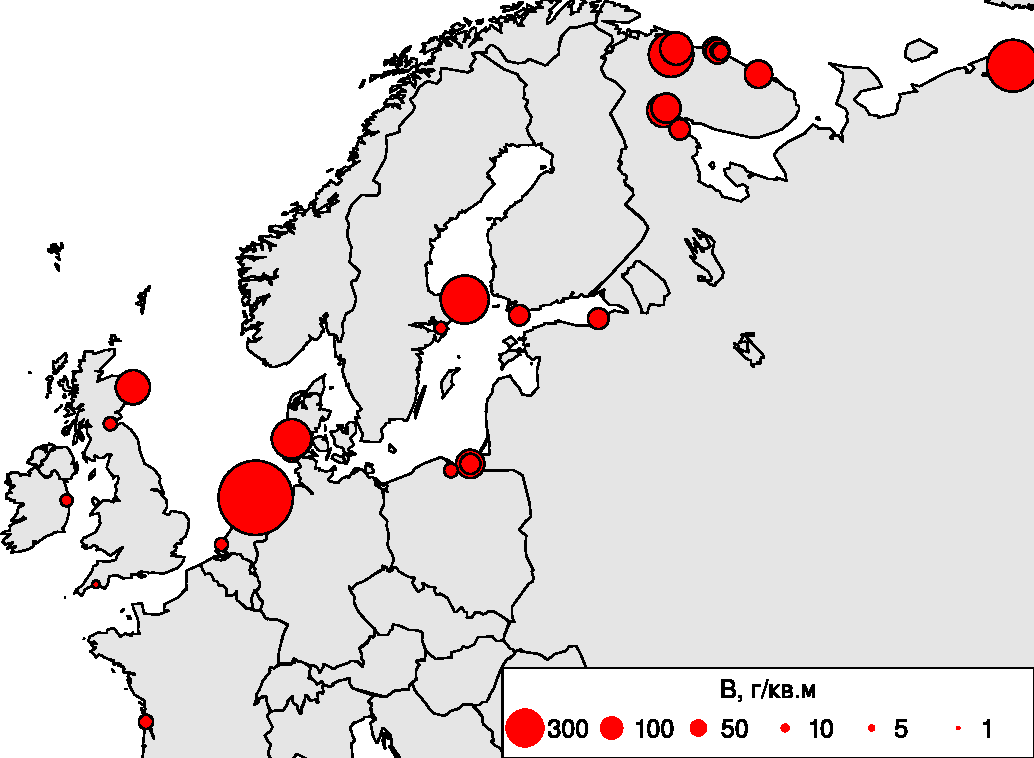
\includegraphics[width=.9\textwidth]{Bmean_ru1.pdf}\\[1ex]
			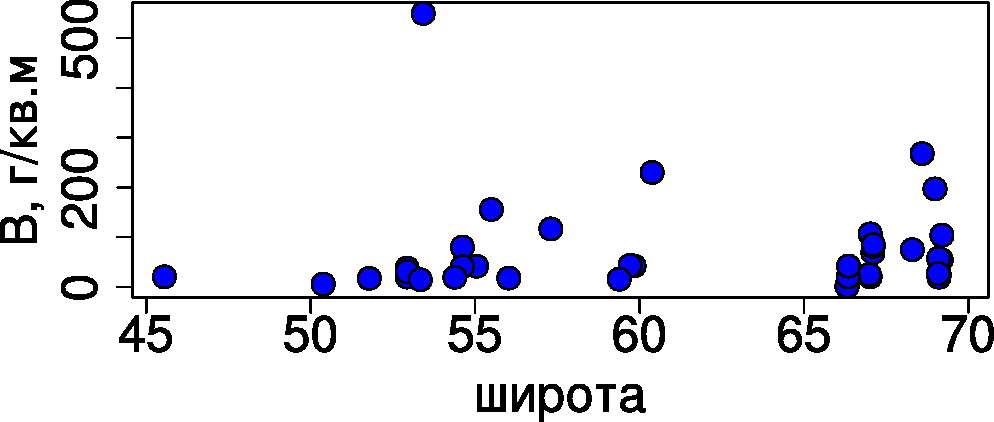
\includegraphics[width=.9\textwidth]{lat_vs_Bmean_big1.pdf}\\
{\scriptsize Корреляция Спирмена: $r_{s} = -0,3$, $p < 0,06$.}
		\end{center}
	\end{minipage}

{\tiny Средние значения показателей пропорциональны площади круга на карте}
\end{frame}



%%%%%%%%%%%%%%%%%%%%%%%%%%%%%%%%%%%%%%%%%%%%%%%%%%%%%
		\section[Динамика численности]{Динамика плотности поселений {\it Macoma balthica} в Белом море}
%%%%%%%%%%%%%%%%%%%%%%%%%%%%%%%%%%%%%%%%%%%%%%%%%%%%%
\begin{frame}{\insertpagenumber.\ Динамика плотности поселений {\it M.~balthica} в вершине Кандалакшского залива}
	\begin{minipage}[t]{.49\linewidth}
		\begin{center}
			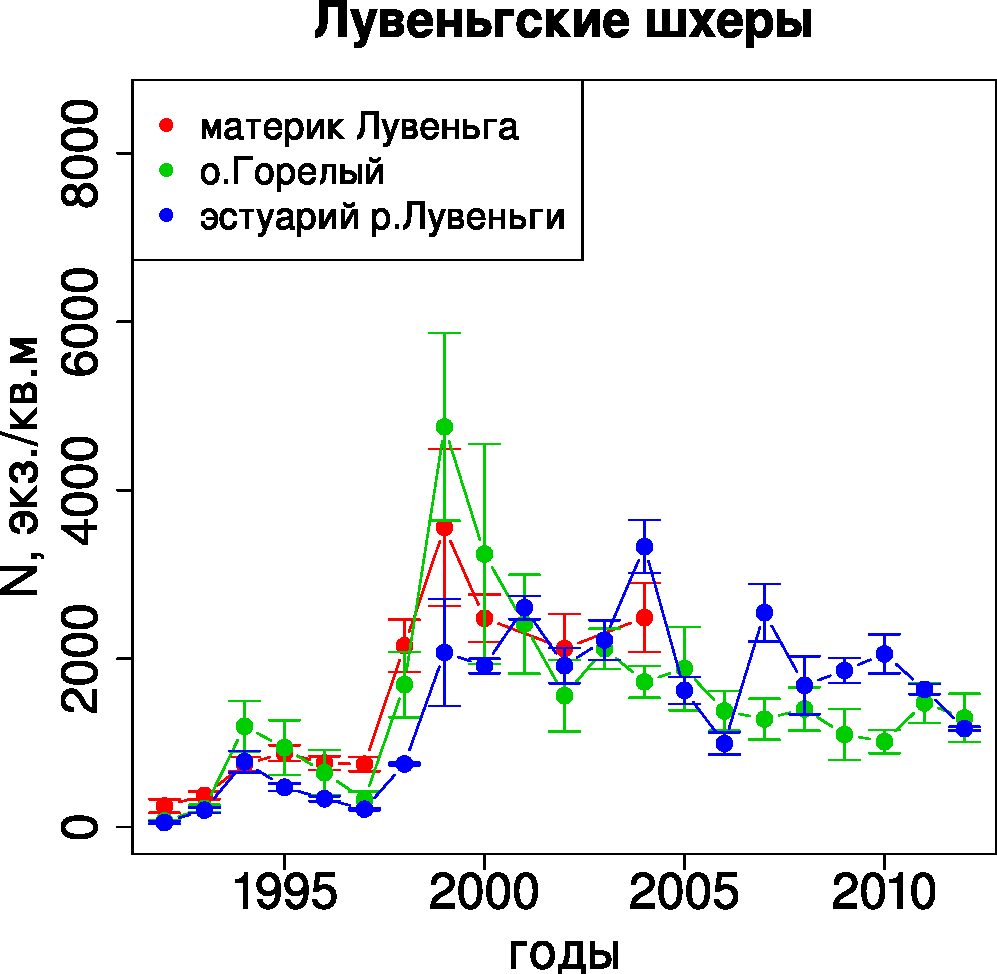
\includegraphics[width=\textwidth]{N2_dynamic_Luvenga_big1.pdf}
		\end{center}
	\end{minipage}
%
	\begin{minipage}[t]{.49\linewidth}
		\begin{center}
			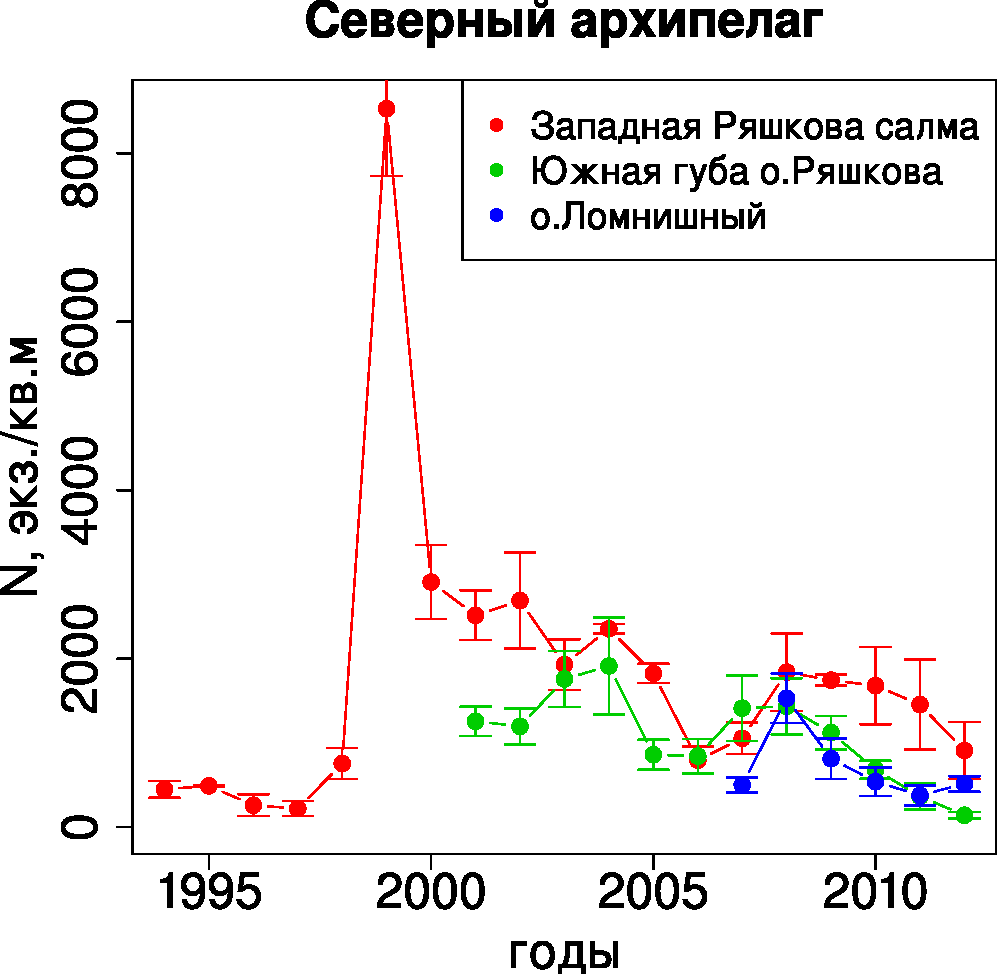
\includegraphics[width=\textwidth]{N2_dynamic_North_big1.pdf}
		\end{center}
	\end{minipage}
{\tiny По оси ординат указана средняя плотность поселения без учета спата}
\end{frame}

\begin{frame}{\insertpagenumber.\ Синхронность динамики плотности поселений {\it M.~balthica} в Кандалакшском заливе Белого моря}
		\begin{center}
%			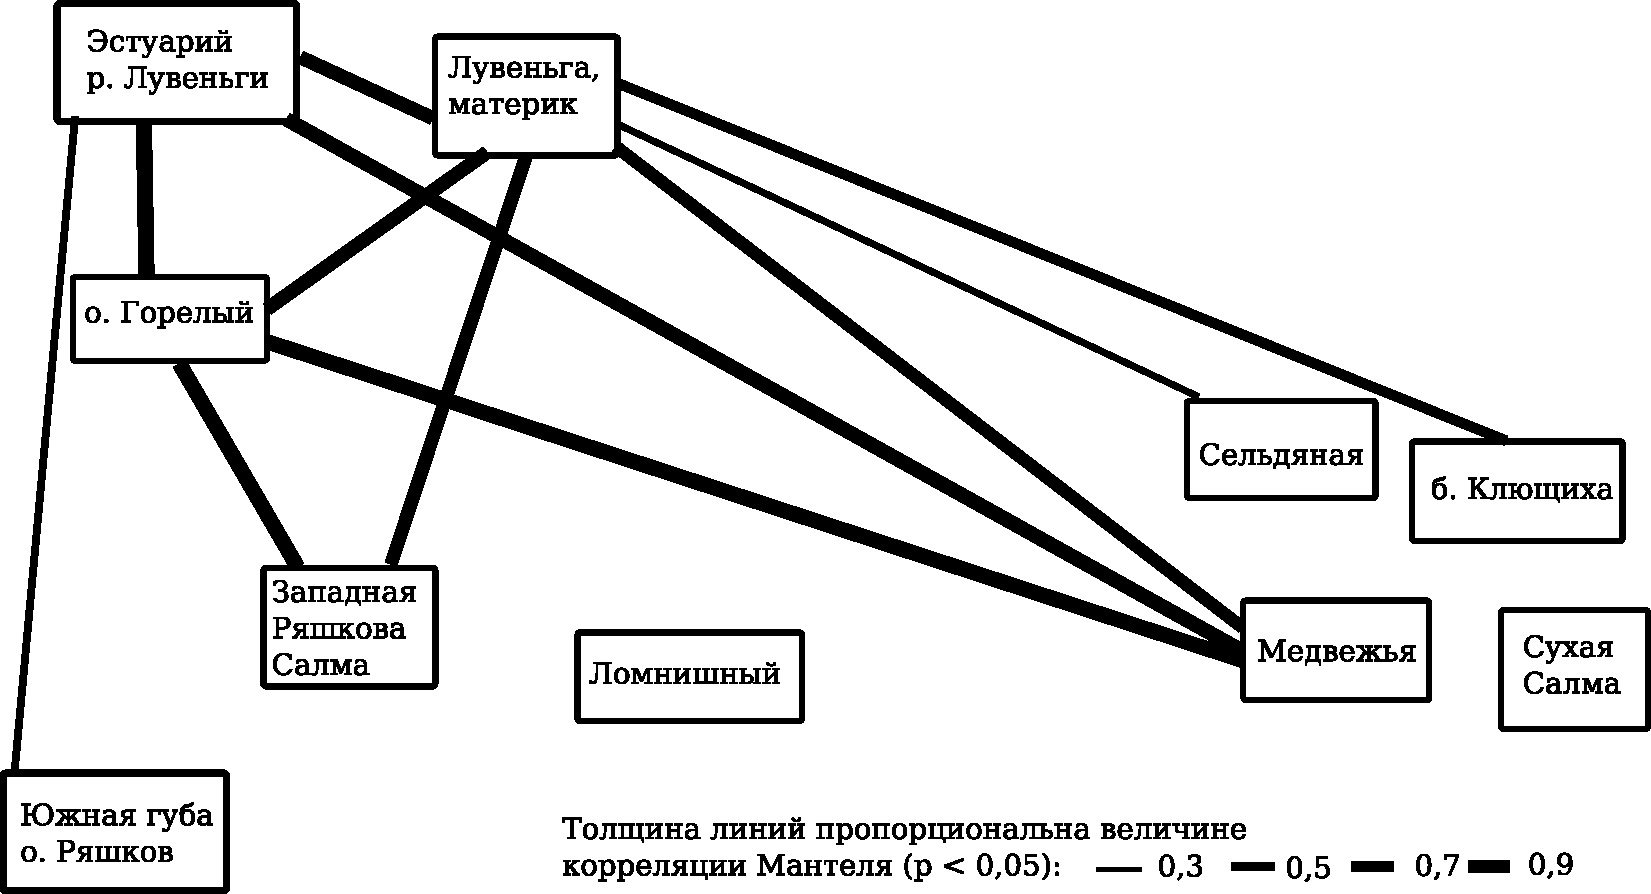
\includegraphics[width=\textwidth]{mantel1.pdf}
			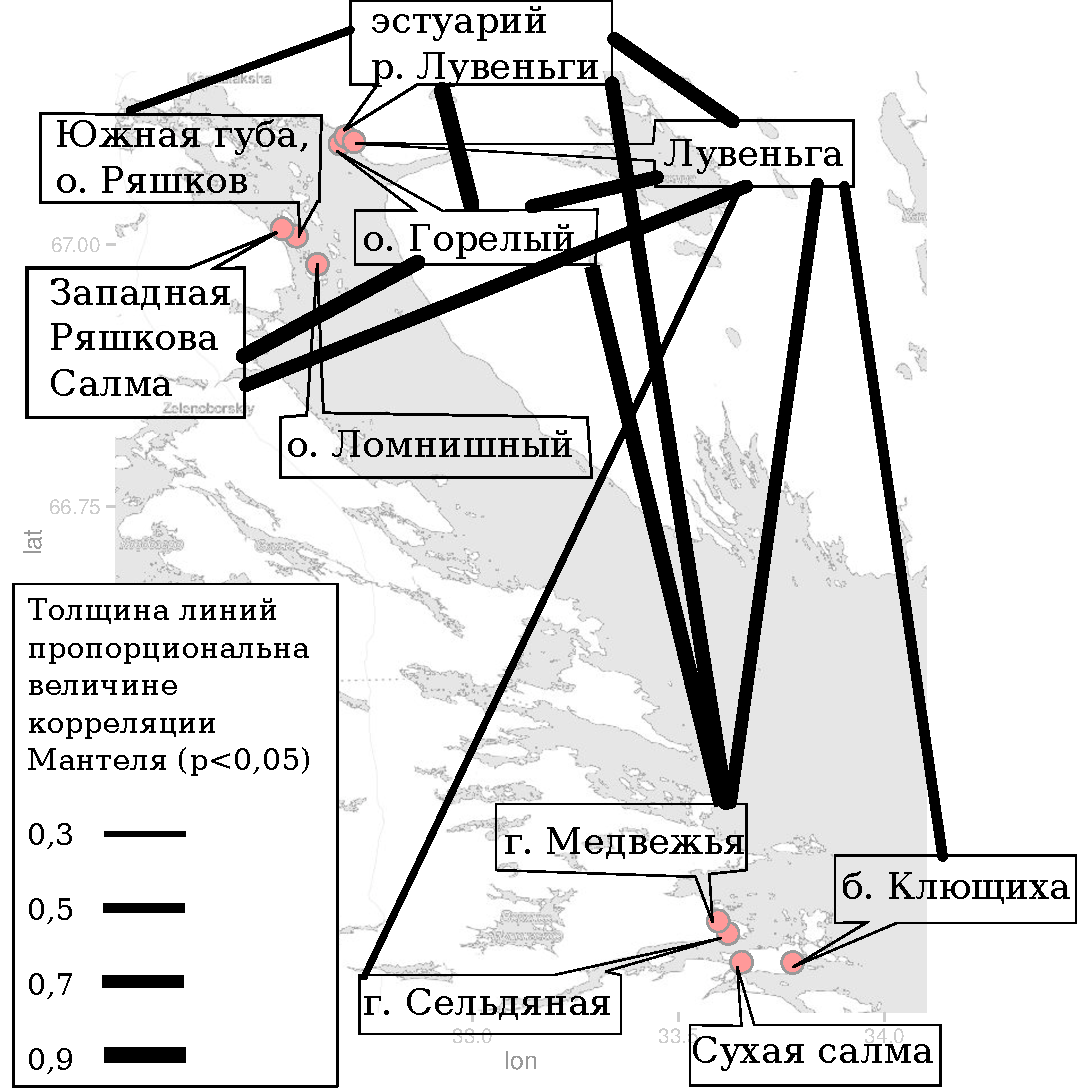
\includegraphics[height=.8\textheight]{mantel_map.pdf}
		\end{center}
\end{frame}


\begin{frame}{\insertpagenumber.\ Моделирование влияния температуры на численность {\it M.~balthica} в Кандалакшском заливе Белого моря}
\begin{center}
{\large $\ln(N_{t1}) = 1,96 + 0,60 \times \ln(N_{t}) - 0,09 \times T_{wt1}$}
\end{center}
{\scriptsize $F = 37,04$; $p < 0,0001$. $R^2 = 0,6$.} \\
	\begin{minipage}[t]{.49\linewidth}
		\begin{center}
			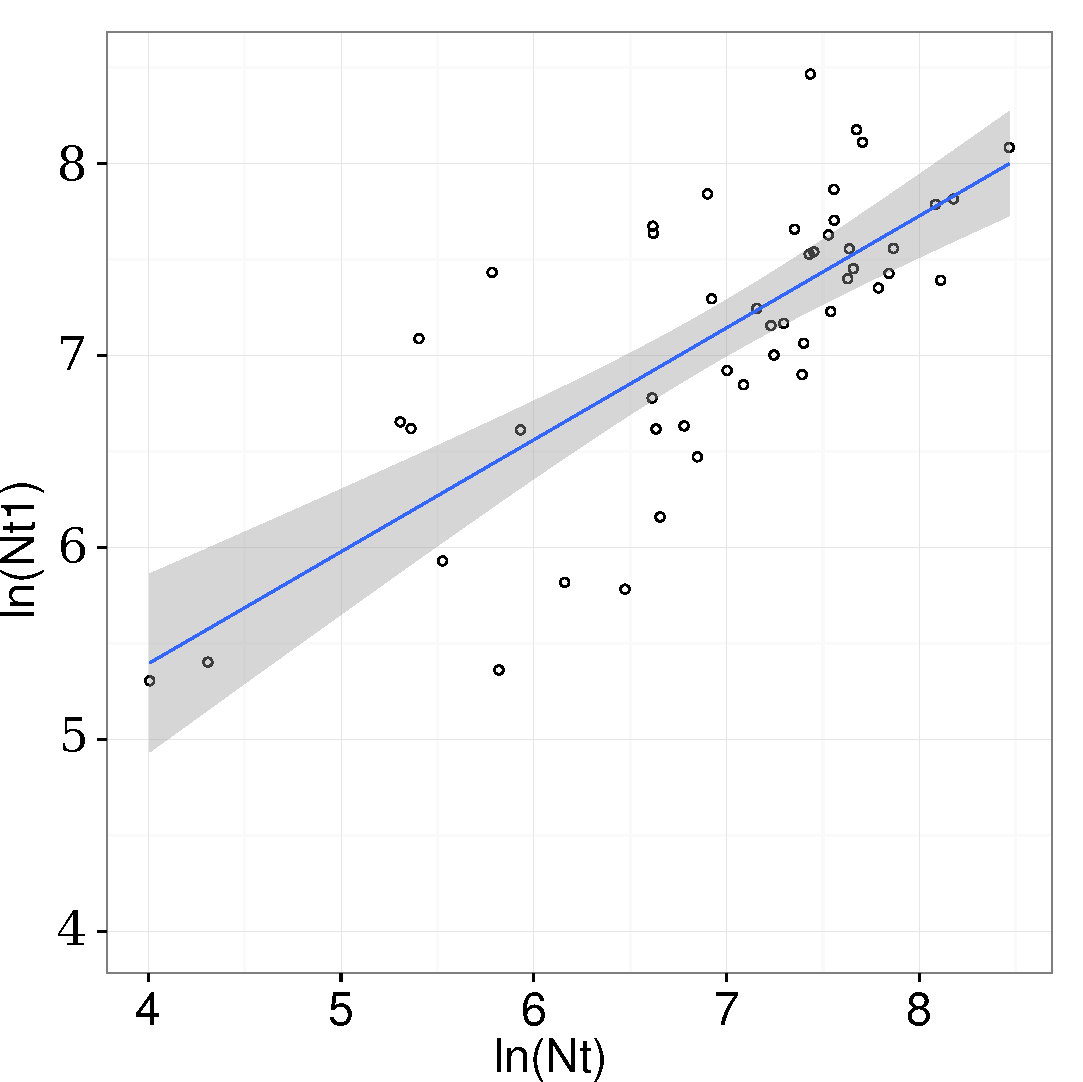
\includegraphics[width=.79\textwidth]{./lodNt_vs_logNt1_2.pdf}
		\end{center}
	\end{minipage}
%
	\begin{minipage}[t]{.49\linewidth}
		\begin{center}
			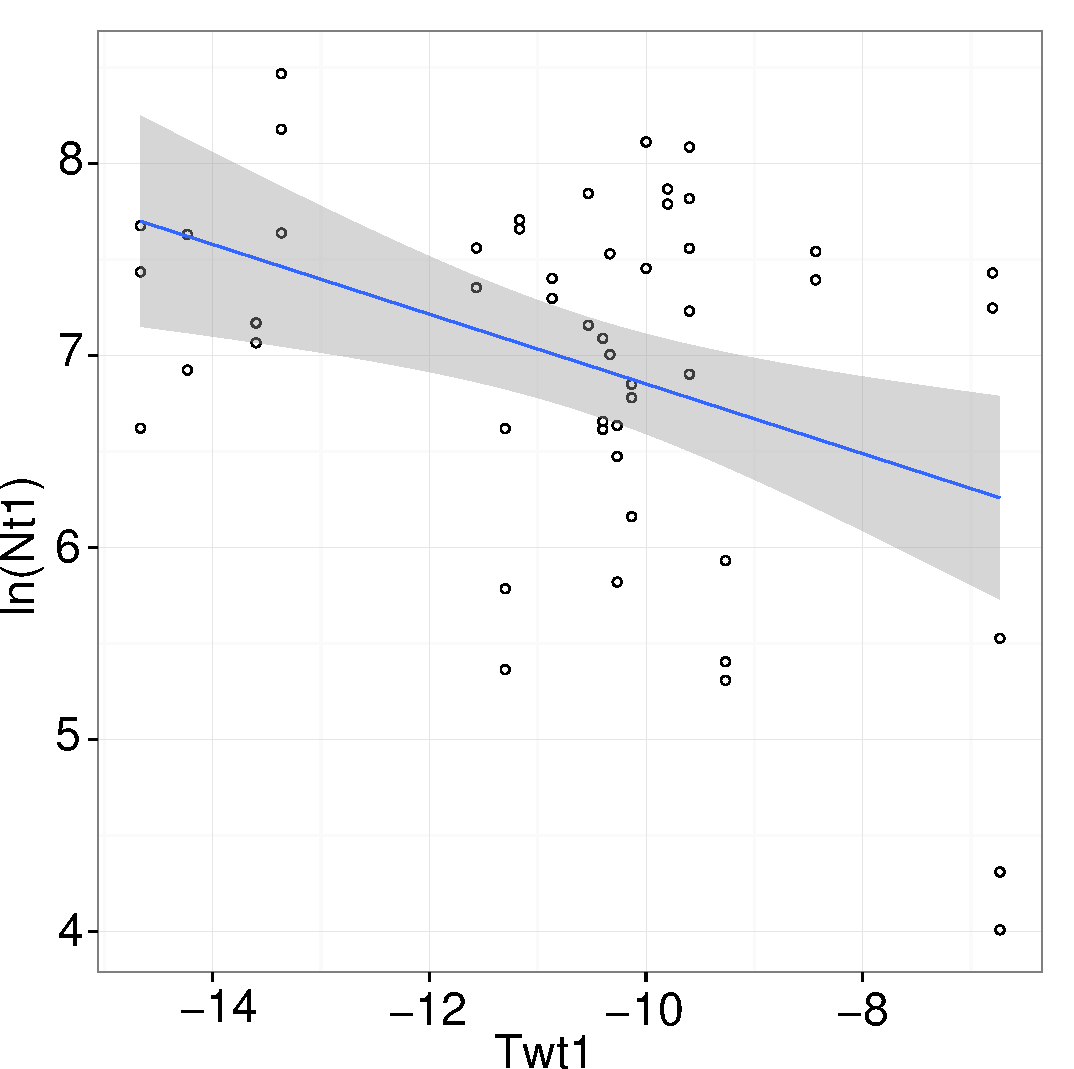
\includegraphics[width=.79\textwidth]{./Twt1_vs_logNt1_2.pdf}
		\end{center}
	\end{minipage}
{\tiny $\log(N_{t1})$ и $\log(N_{t})$~--- логарифм средней численности маком в данный ($t1$) и предыдущий ($t$) годы; $T_{wt1}$~--- среднезимняя температура в текущий год.}
\end{frame}

%%%%%%%%%%%%%%%%%%%%%%%%%%%%%%%%%%%%%%%%%%%%%%%%%%%%%
		\section[Размерная структура]{Характер размерной структуры поселений {\it Macoma balthica}}
%%%%%%%%%%%%%%%%%%%%%%%%%%%%%%%%%%%%%%%%%%%%%%%%%%%%%

\begin{frame}{\insertpagenumber.\ Динамика размерной структуры}
Тип 1: чередование вариантов распределения\\
Пример: эстуарий р.~Лувеньги\\

			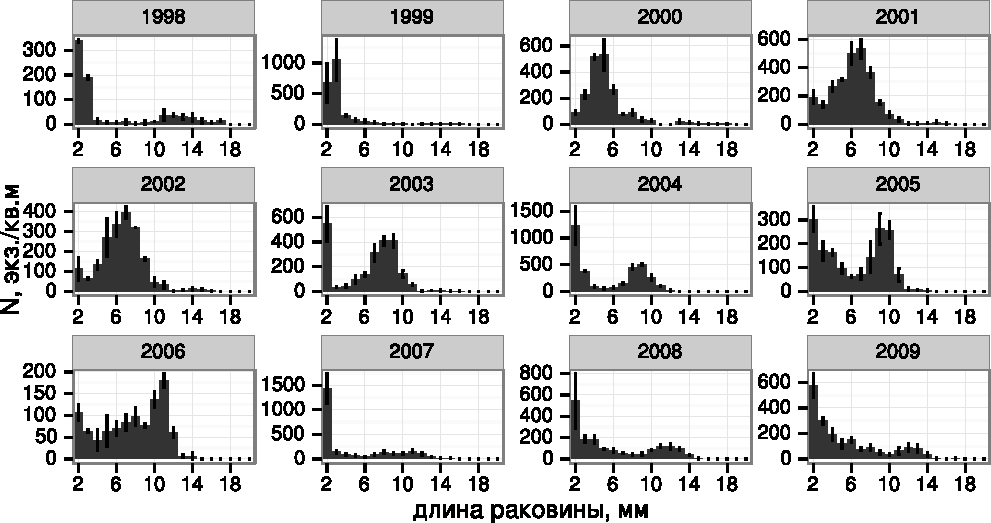
\includegraphics[height=.78\textheight]{Estuary_total_size_oneplot_nonscale1.pdf}\\
\end{frame}



\begin{frame}{\insertpagenumber.\ Динамика размерной структуры}
Тип 2: ежегодное повторение мономодального распределения\\
Пример: Южная губа острова Ряшкова\\

			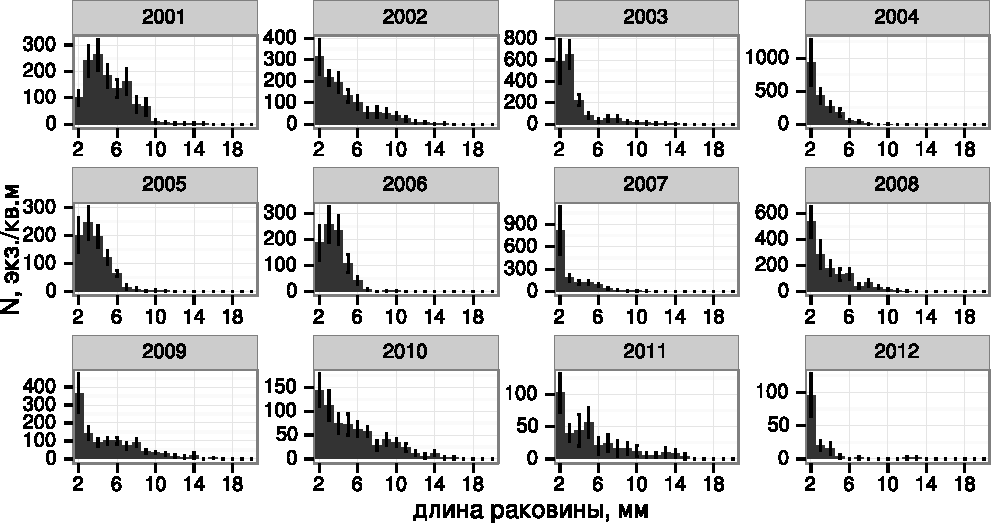
\includegraphics[height=.78\textheight]{YuG_sizestr_oneplot_nonscale1.pdf}
\end{frame}



\begin{frame}{\insertpagenumber.\ Варианты организации поселений {\it M.~balthica}}
	\begin{minipage}[t]{.3\linewidth}
		\begin{center}
	\textcolor{red}{Чередование типов\\ размерной структуры} \\ 6 поселений \\
			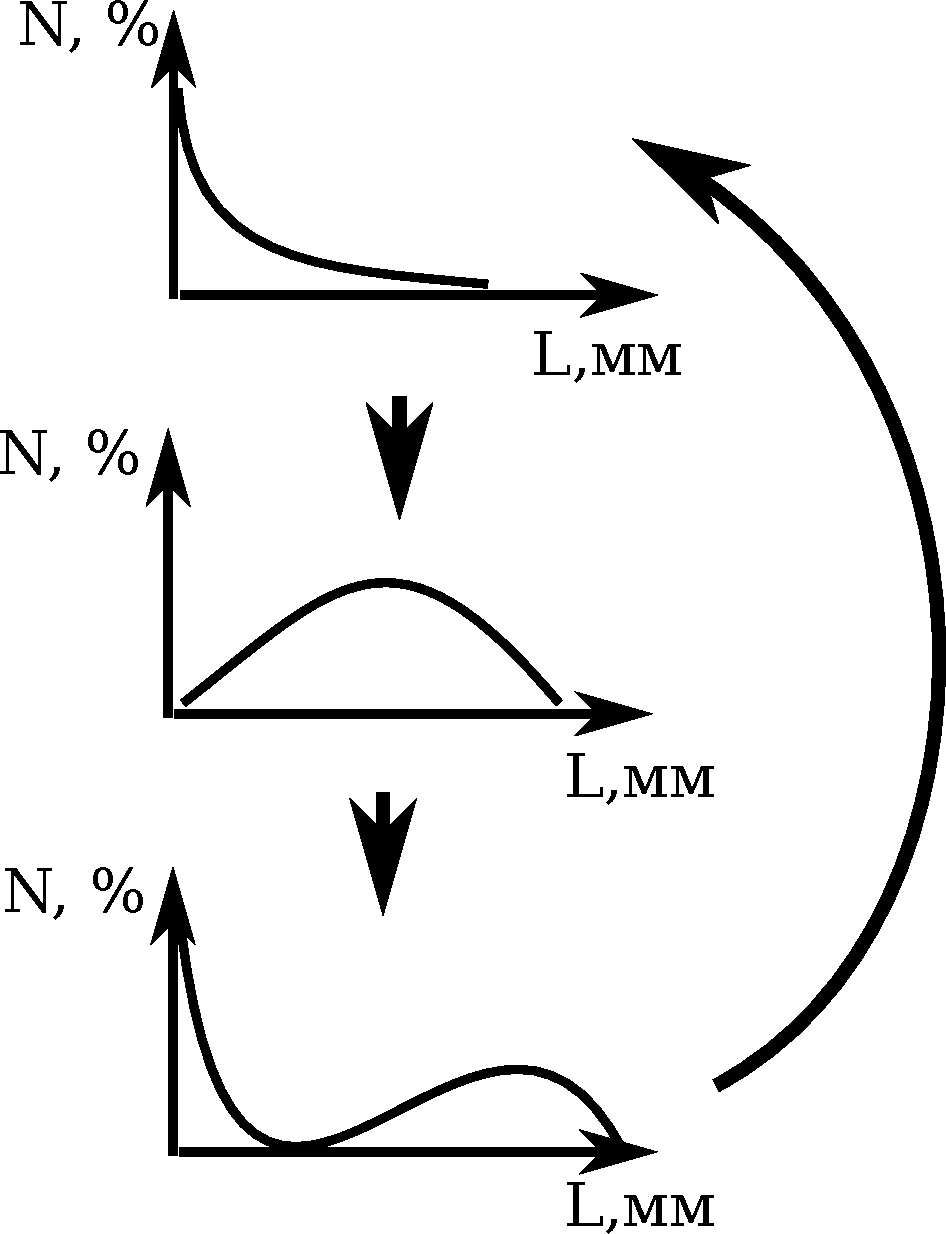
\includegraphics[width=\textwidth]{Dymanic_cheredovanie.pdf}
		\end{center}
\textcolor{red}{\scriptsize +поселение в г.~Дальне-Зелененцкой Баренцева моря}
	\end{minipage}
%
	\begin{minipage}[t]{.35\linewidth}
		\begin{center}
			{\small Распространение поселений с разной организацией в Кандалакшском заливе Белого моря}\\
			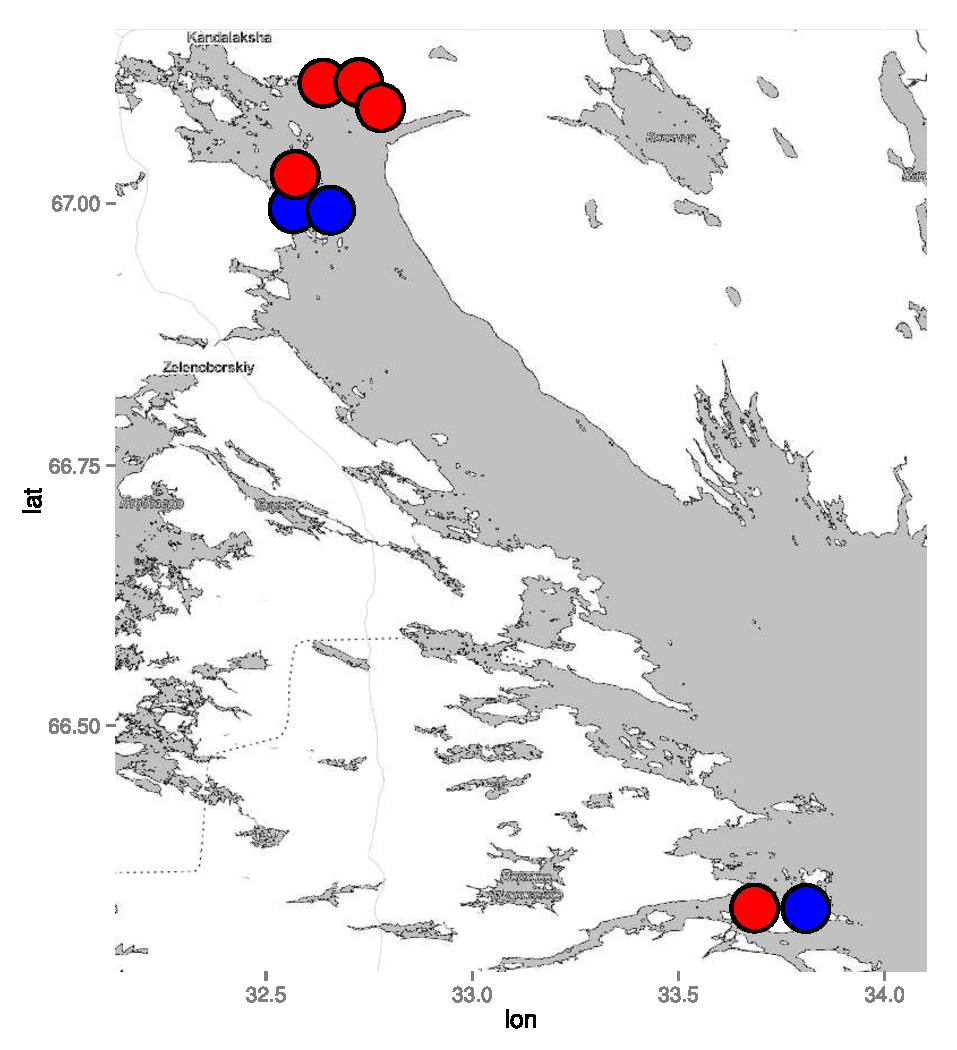
\includegraphics[width=\textwidth]{map_size_distr.pdf}
		\end{center}

	\end{minipage}
%
	\begin{minipage}[t]{.3\linewidth}
		\begin{center}
\textcolor{blue}{Ежегодное повторение\\ размерной структуры }\\ 3 поселения \\
			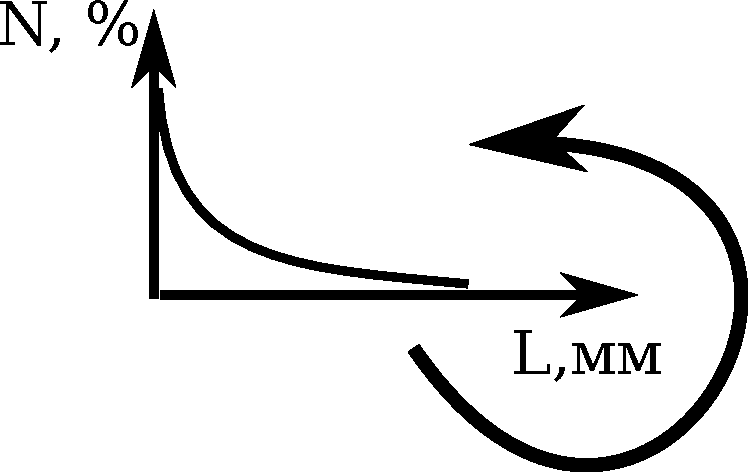
\includegraphics[width=.8\textwidth]{Dymanic_povtorenie.pdf}\\
		\end{center}
\begin{scriptsize}
	\begin{itemize}
		\item сходный гранулометрический состав грунта
		\item воздействие хищников?
	\end{itemize}
\end{scriptsize}
	\end{minipage}
\end{frame}

%%%%%%%%%%%%%%%%%%%%%%%%%%%%%%%%%%%%%%%%%%%%%%%%%%%%%
		\section[Линейный рост]{Линейный рост {\it Macoma balthica}}
%%%%%%%%%%%%%%%%%%%%%%%%%%%%%%%%%%%%%%%%%%%%%%%%%%%%%

\begin{frame}{\insertpagenumber.\ Широтные изменения скорости роста {\it M.~balthica} в европейской части ареала}

{\footnotesize Коэффициент $\omega = L_{max} \times k$ (Appeldoorn, 1983; Beukema, Meehan, 1985)}
		\begin{center}
			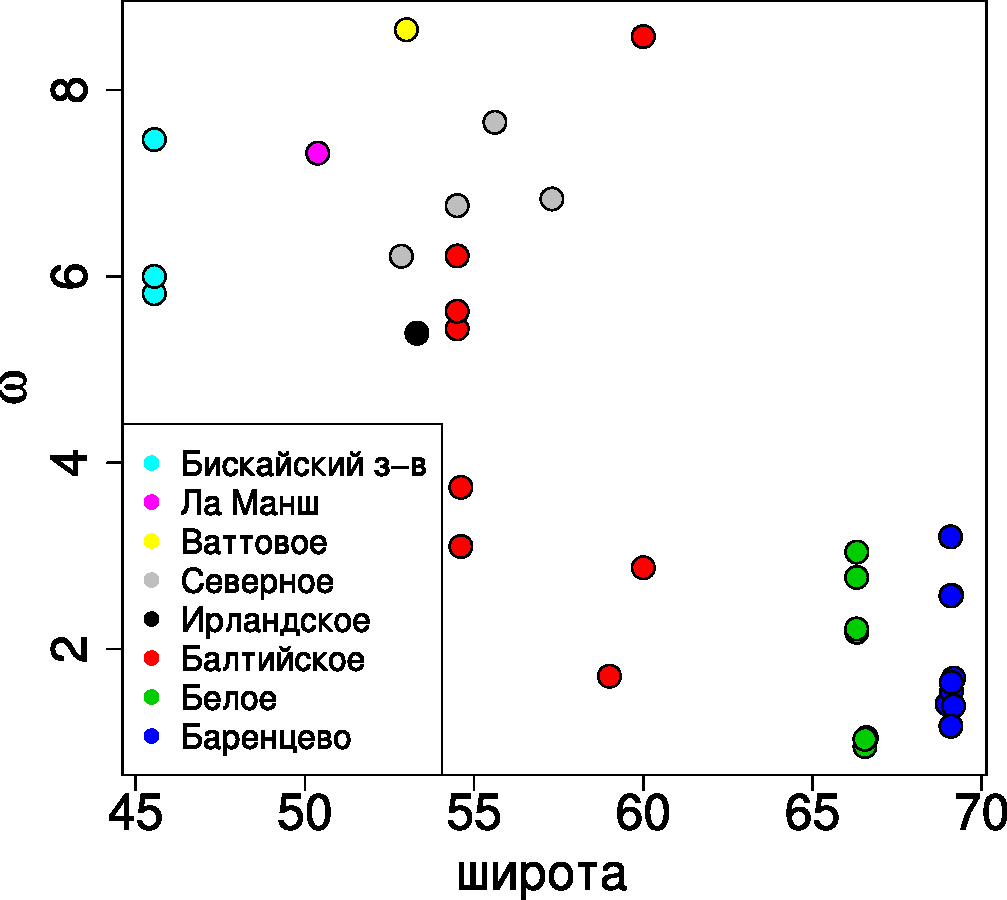
\includegraphics[height=.68\textheight]{./long_vs_omega_big1.pdf}
		\end{center}
{\footnotesize Корреляция Спирмена: $r_{s} = -0,60$, $p < 0,0001$.}

\end{frame}

\begin{frame}{\insertpagenumber.\ Линейный рост {\it M.~balthica} в европейской части ареала}
	\begin{minipage}[t]{.52\linewidth}
		\begin{center}
			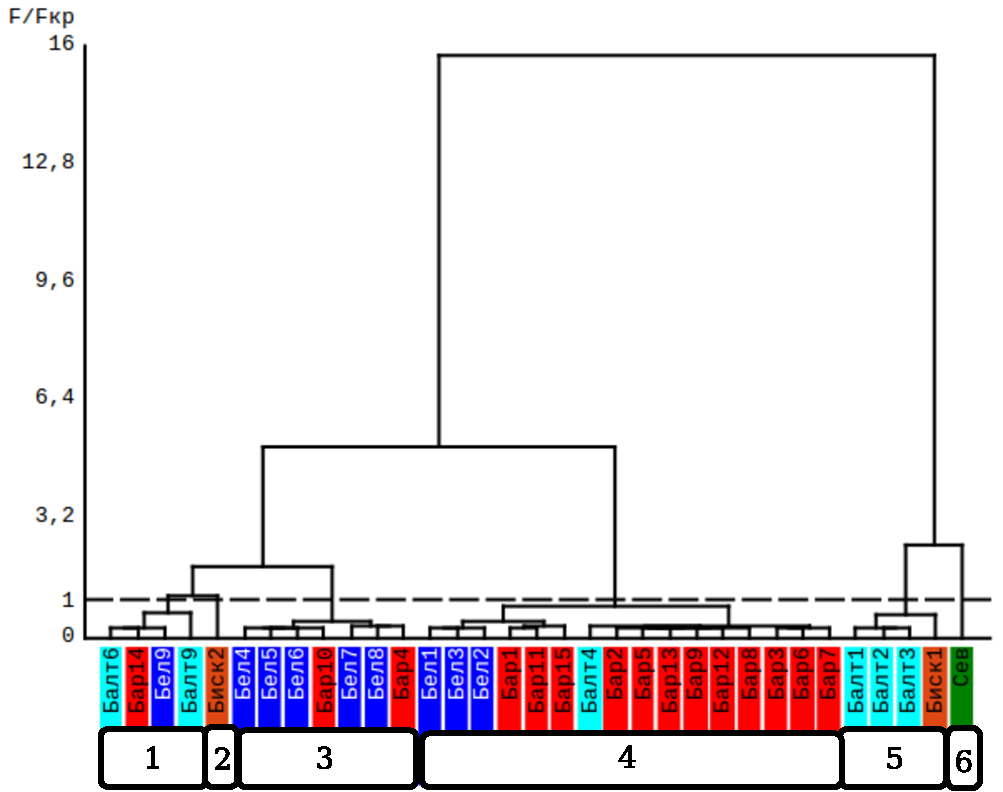
\includegraphics[width=\textwidth]{./Europe_clusters_usrednenie.pdf}
		\end{center}

Цветовые обозначения: \textcolor{red}{Баренцево море}, 
\textcolor{blue}{Белое море}, 
\textcolor{cyan}{Балтийское море}, 
\textcolor{green}{Северное море}, 
\textcolor{brown}{Бискайский залив}.
	\end{minipage}
%
	\begin{minipage}[t]{.45\linewidth}
		\begin{center}
			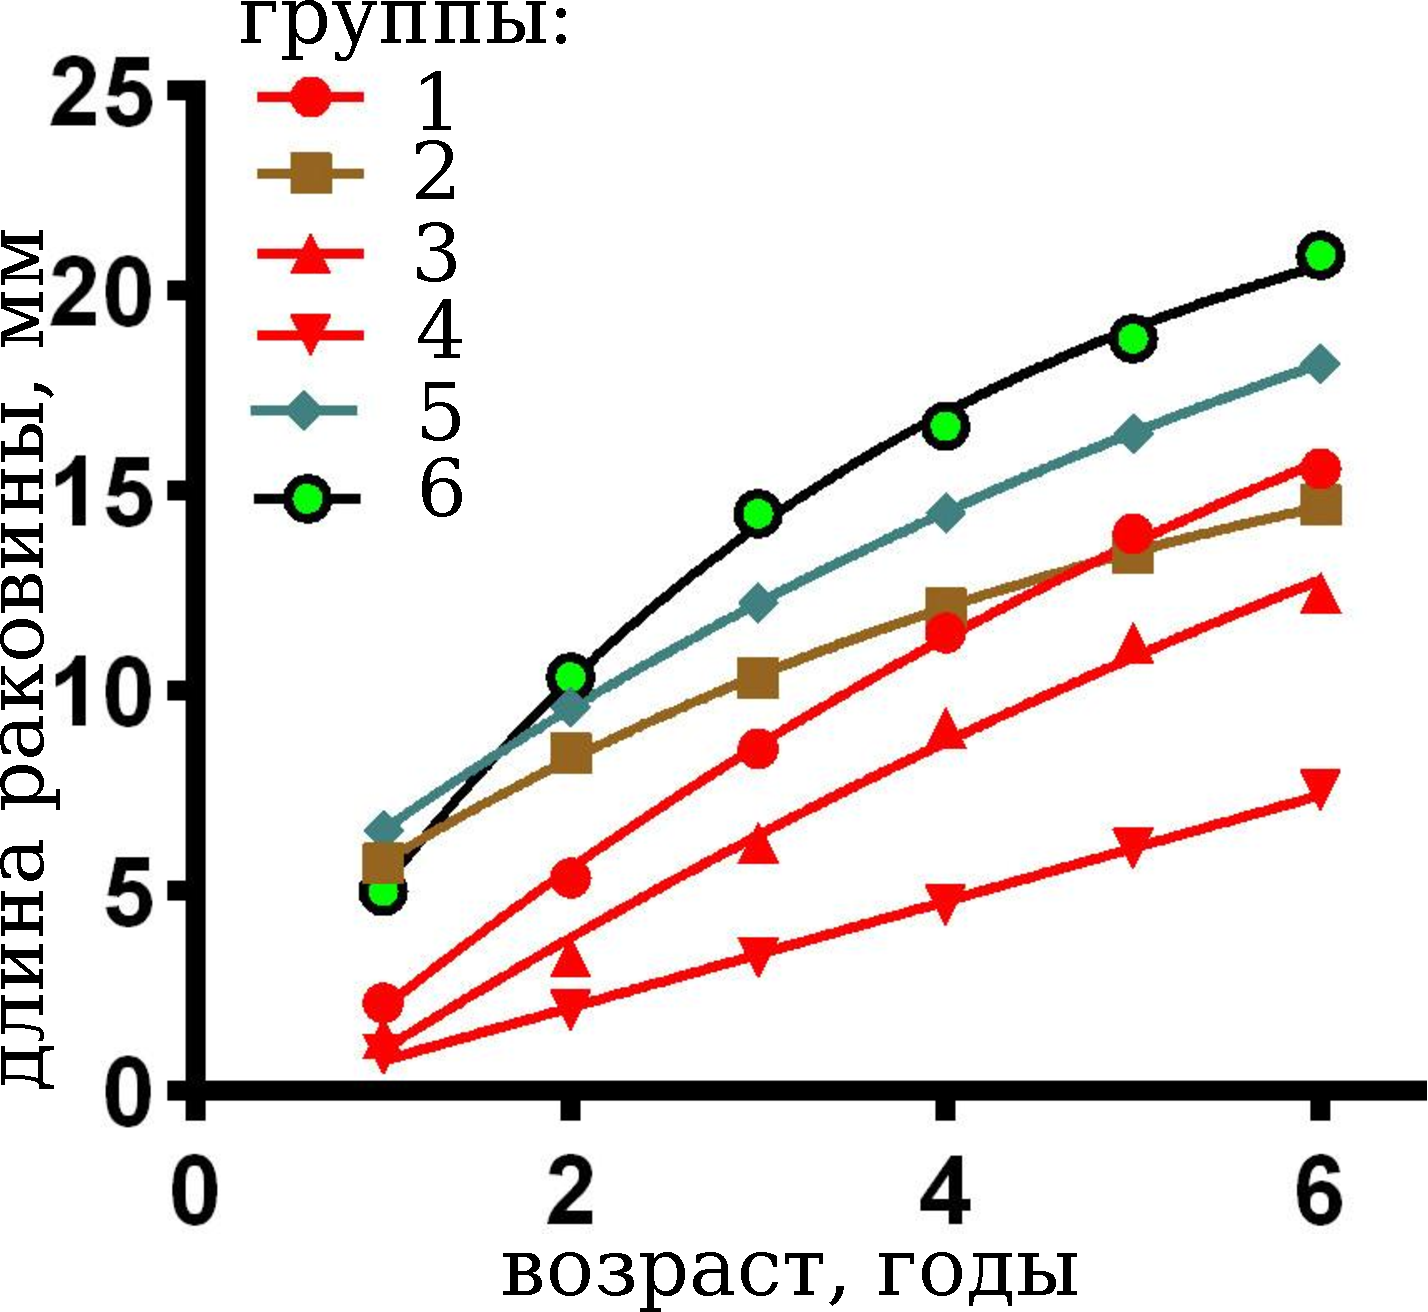
\includegraphics[width=\textwidth]{./Europe_growth_groups_prizm.pdf}
		\end{center}
	\end{minipage}
\end{frame}

%\begin{frame}{\small Изменения среднего годового прироста особей {\it M.~balthica} в зависимости от начальной средней длины их раковин, мареографического уровня обитания (A) и условного смещения участка по побережью Мурмана на восток (Б)}
%	\begin{minipage}[t]{.49\linewidth}
%				{\small А}
%			\begin{center}
%				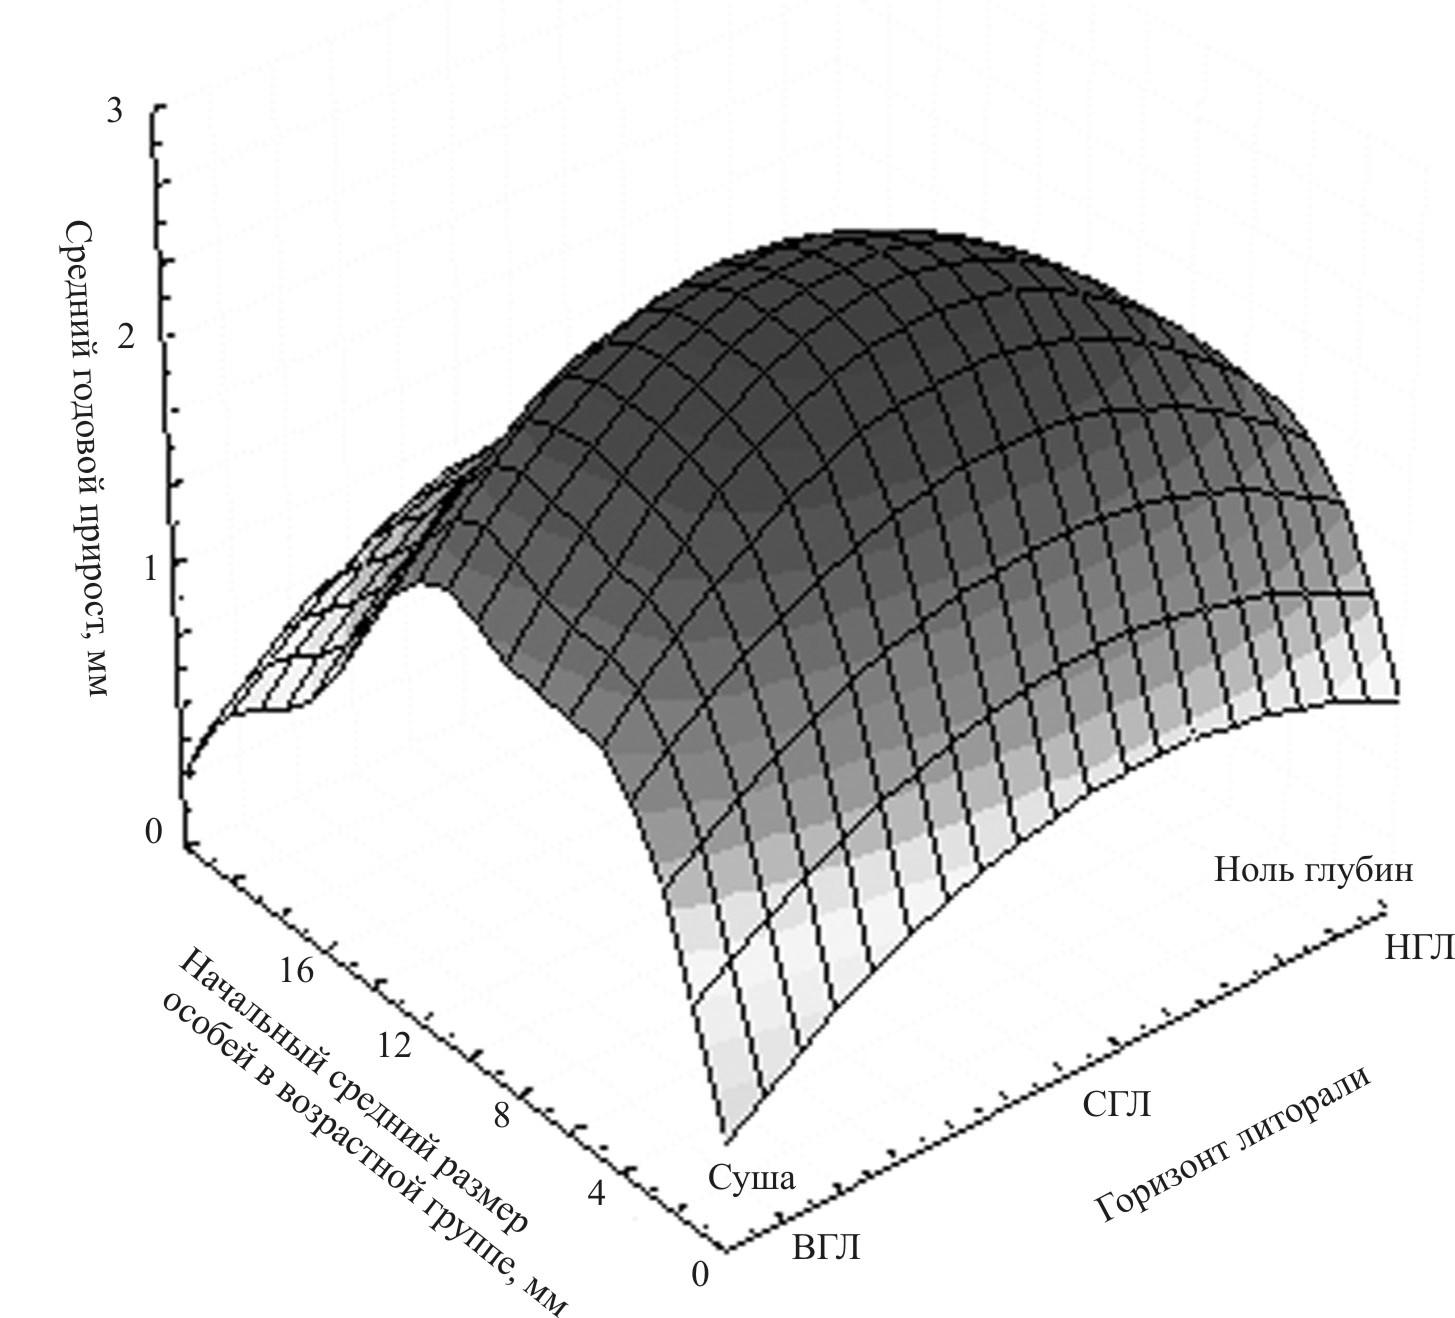
\includegraphics[width=\textwidth]{./prirost_otklik_mareography.jpg}
%			\end{center}
%		\end{minipage}
%	\hfil %Это пружинка отодвигающая рисунки друг от друга
%		\begin{minipage}[t]{.49\linewidth}
%				{\small Б}
%			\begin{center}
%				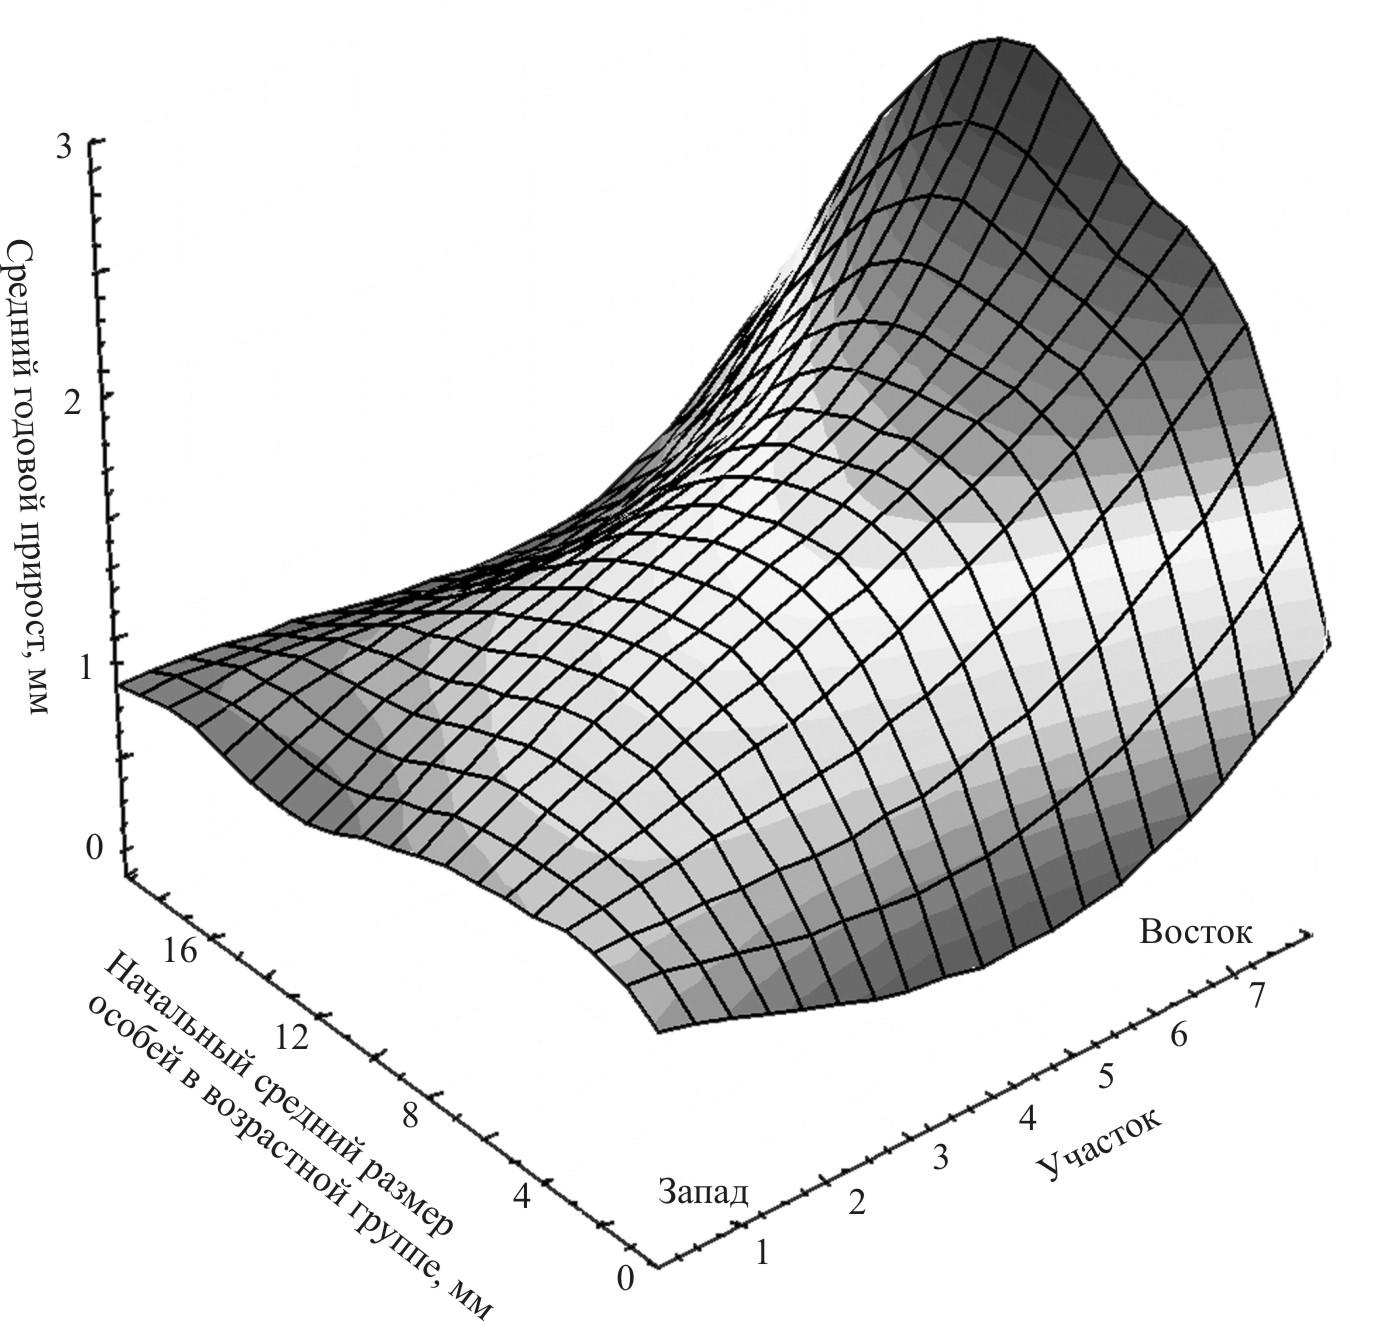
\includegraphics[width=\textwidth]{./prirost_otklik_geography.jpg}
%			\end{center}
%		\end{minipage}
%\tiny{1~--- Абрам-мыс, 2~--- Пала-губа, 3~--- Гаврилово, 4~--- Ярнышная, 5~--- Дальнезеленецкая, 6~--- Шельпино, 7~--- Порчниха.\\
%Горизонты литорали: ВГЛ~--- верхний, СГЛ~--- средний, НГЛ~--- нижний.}
%\end{frame}


%%%%%%%%%%%%%%%%%%%%%%%%%%%%%%%%%%%%%%%%%%%%%%%%%%%%%
		\section[Оседание]{Режим формирования спата}
%%%%%%%%%%%%%%%%%%%%%%%%%%%%%%%%%%%%%%%%%%%%%%%%%%%%%
\begin{frame}{\insertpagenumber.\ Обилие спата \textit{Macoma balthica}}
		\begin{center}
			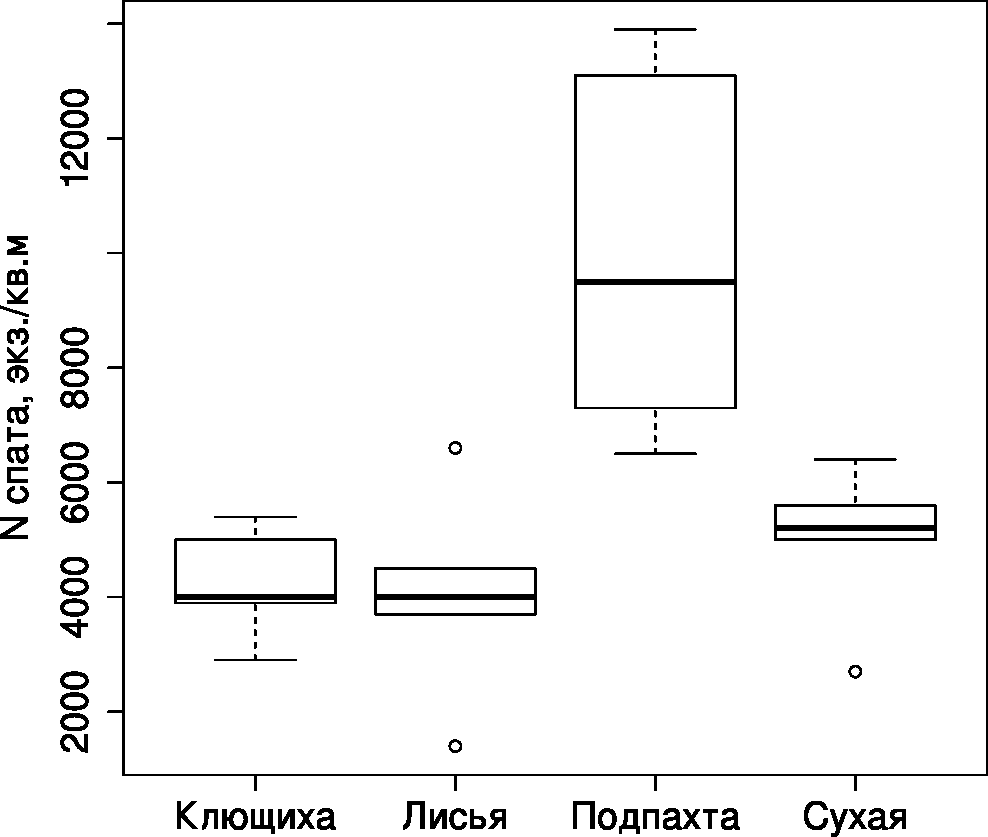
\includegraphics[height=.8\textheight]{N_spat1.pdf}
		\end{center}
\end{frame}



%%%%%%%%%%%%%%%%%%%%%%%%%%%%%%%%%%%%%%%%%%%%%%%%%%%%%
		\section{Выводы}
%%%%%%%%%%%%%%%%%%%%%%%%%%%%%%%%%%%%%%%%%%%%%%%%%%%%%

\begin{frame}{\insertpagenumber.\ Выводы}
	\begin{scriptsize}
\addtocounter{enumi}{0}
	\begin{enumerate}
		\item В Кольском заливе Баренцева моря и Кандалакшском заливе  Белого моря значения биомассы (до 200 г/м$^2$) поселений {\it Macoma balthica} сопоставимы с аналогичным показателем в европейской части ареала, а плотность поселений нередко оказывается выше (до 8~тыс.~экз./м$^2$). Для литорали восточной части Мурманского побережья Баренцева моря типичны поселения {\it M.~balthica} с численностью менее 100 экз./м2 
		\item Плотность поселений спата {\it Macoma balthica} в Белом море может варьировать на порядок в пределах незначительной акватории, и достигать десятков тысяч экз./м$^2$.
		\item Беломорские и баренцевоморские поселения {\it M.~balthica} не различаются по средней скорости роста моллюсков, и отличаются по этому показателю минимальными характеристиками в пределах европейской части ареала вида. 
		\item Динамика размерной структуры поселений {\it Macoma balthica} в Белом и Баренцевом представлена двумя типами. \\
Наболее обычный вариант~--- чередование бимодального и мономодального распределений особей по размерам. При этом первый пик формируют молодые
особи (обычно длиной до 5 мм), а второй модальный класс состоит из взрослых особей (в Белом море длиной 9--12~мм, в Баренцевом море~--- 10--17~мм).
Как относительно редкое событие наблюдается мономодальная структура поселений с ежегодным преобладаем молоди.
		\item Динамика плотности поселений {\it Macoma balthica} в Кандалакшском заливе Белого моря демонстрирует элементы синхронности в поселениях, расположенных на расстоянии от 1 до 100~км, что происходит на фоне резкой межгодовой неравномерности пополнения поселений молодью.  
	\end{enumerate}
	\end{scriptsize}
\end{frame}

		\section*{Благодарности}
{\usebackgroundtemplate{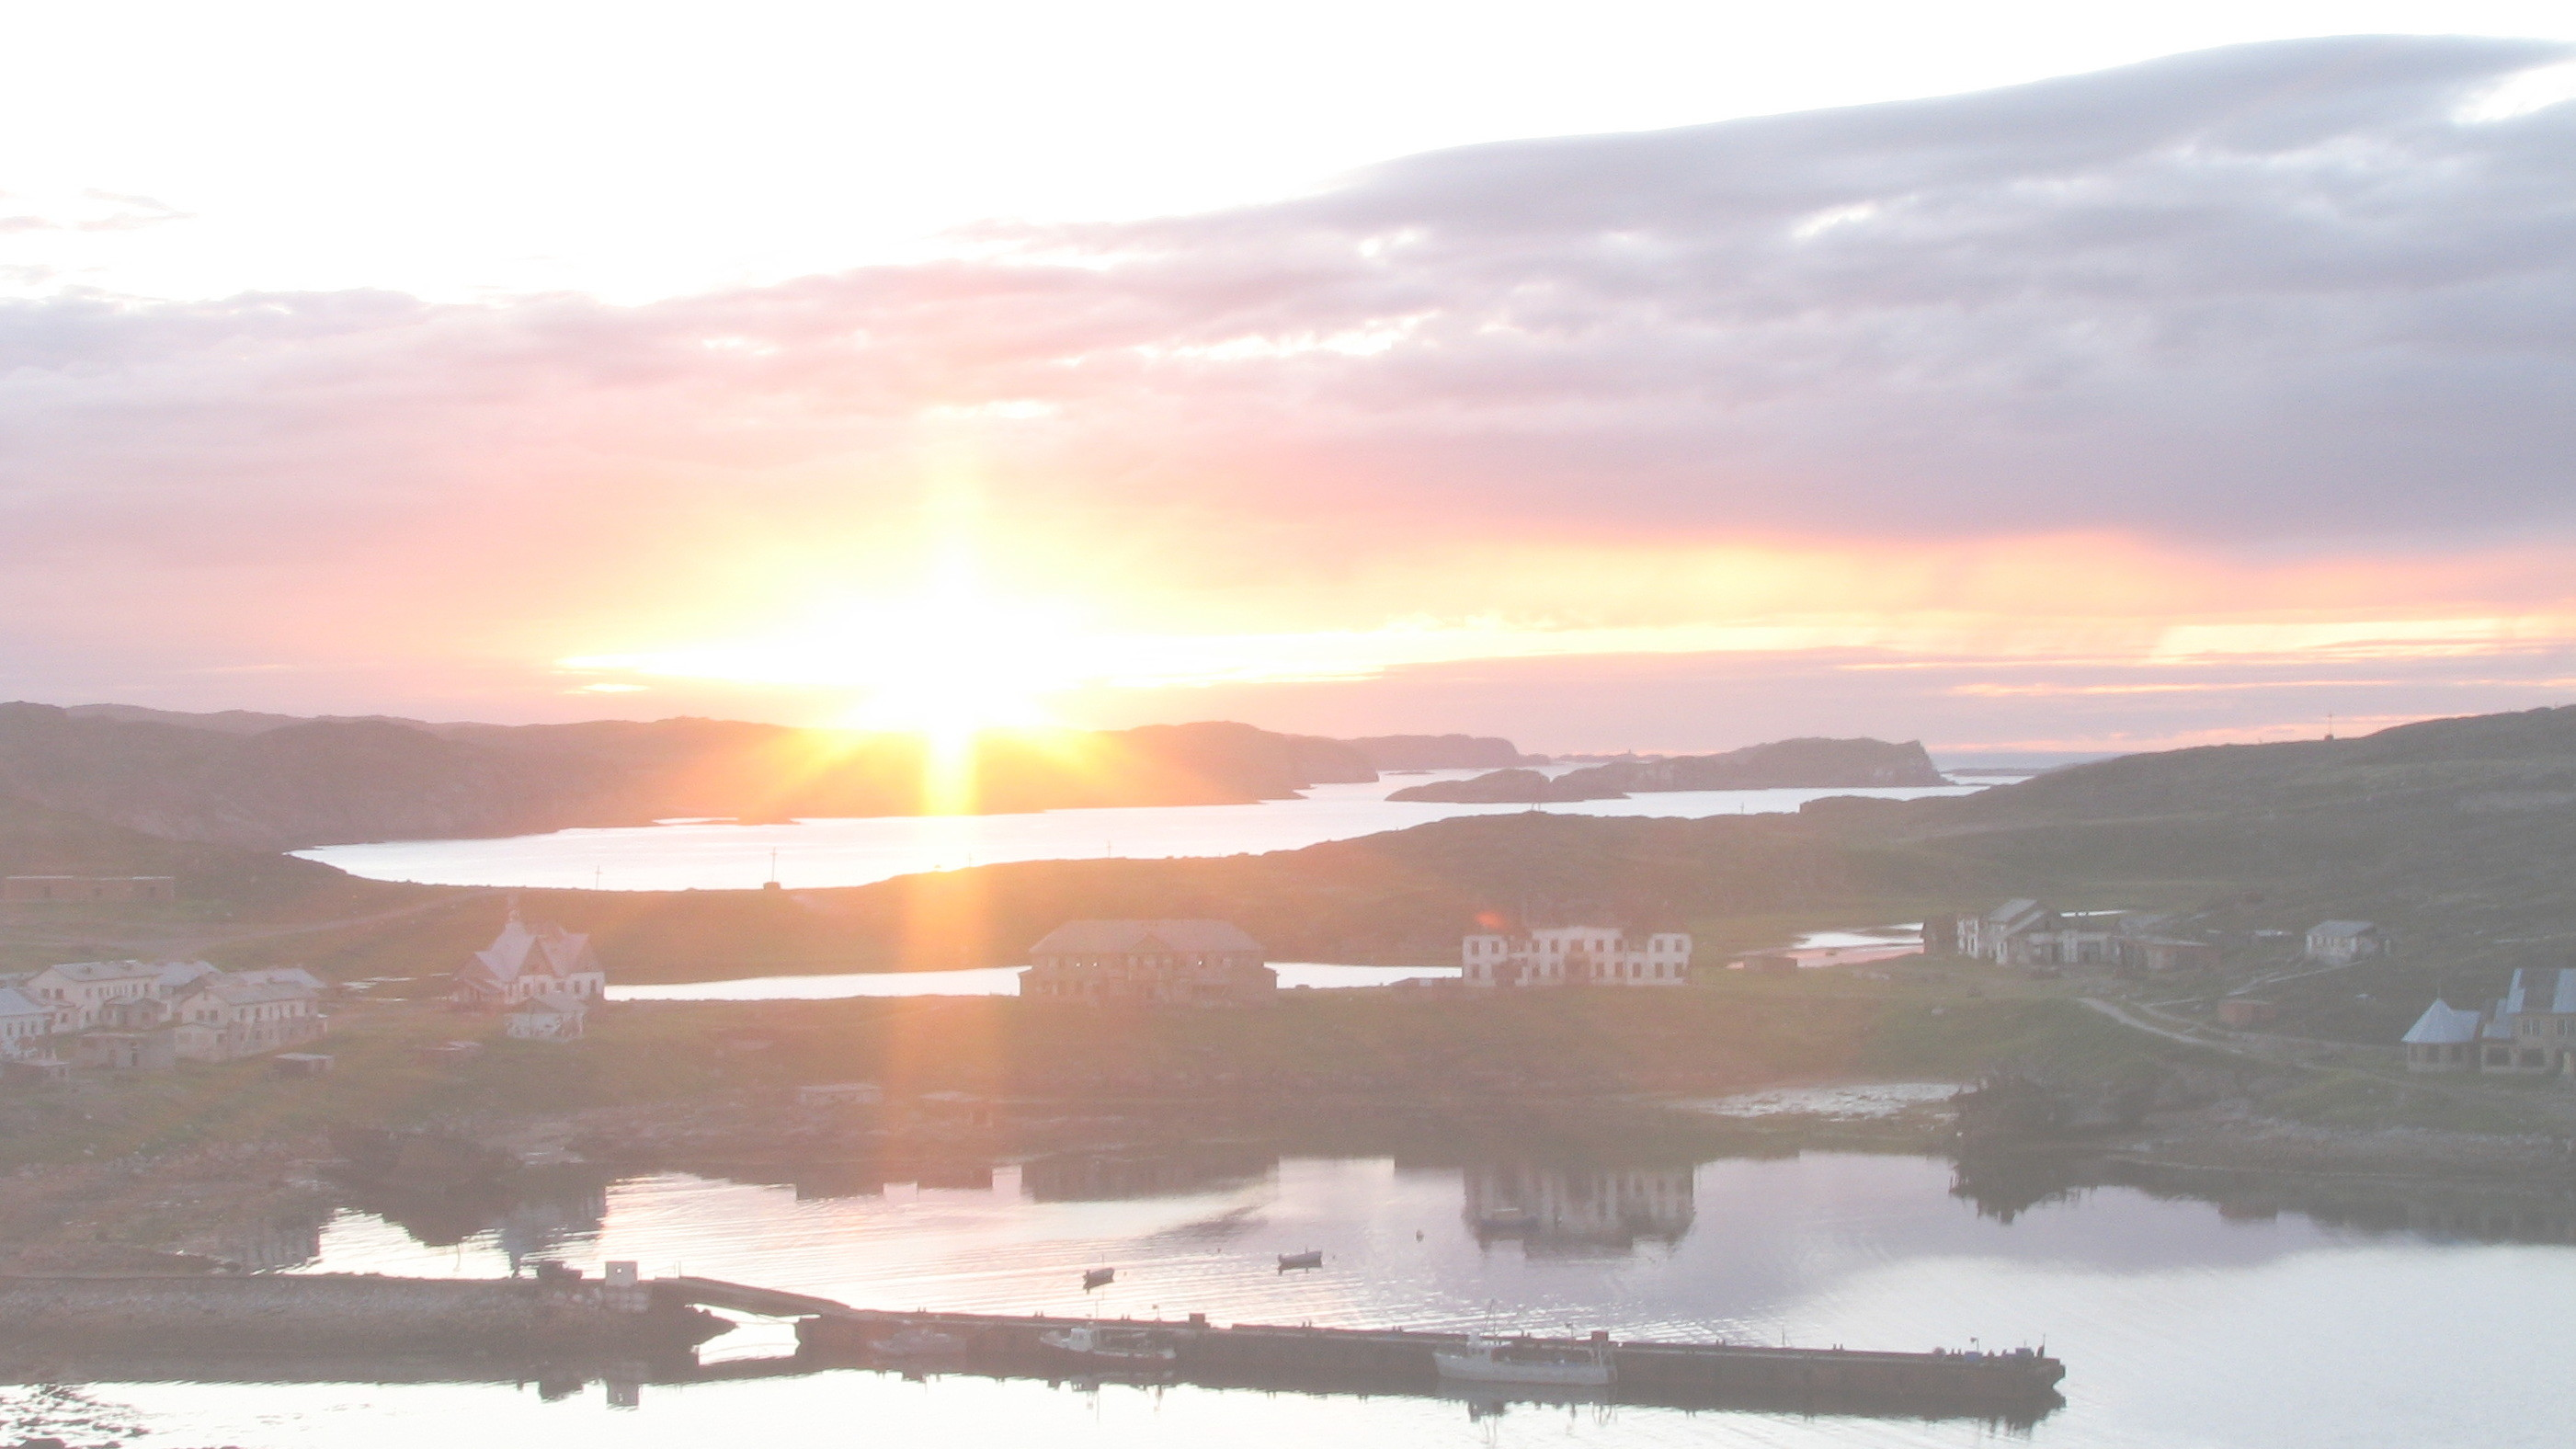
\includegraphics[width=\paperwidth]{fon.JPG}}
\begin{frame}{}
\centering
{\Huge Спасибо за внимание} 
\end{frame}
}

\begin{footnotesize}
\begin{frame}{Благодарности}
	\begin{itemize}
\begin{multicols}{2} [\item научному руководителю Н.\:В.~Максимовичу]

		\item{Д.\:А.~Аристову} 
		\item{Е.\:А.~Генельт-Яновскому}
		\item{А.\:В.~Герасимовой}
		\item{М.В.~Иванову}
		\item{И.\:А.~Коршуновой}
		\item{М.\:В.~Макарову}
		\item{С.\:В.~и С.\:С.~Малавендам}
		\item{А.\:Д.~Наумову}
		\item{А.\:В.~Полоскину}
		\item{И.\:П.~Прокопчук}
		\item{П.\:П.~Стрелкову}
		\item{Ю.\:Ю.~Тамберг}
		\item{О.\:С.~Тюкиной}
		\item{В.\:М.~Хайтову}
		\item{К.\:В.~Шунькиной}
		\item{\fbox{Е.\:А. Нинбургу}}
		\item{\fbox{А.\:С.~Корякину}}
		\item{участникам Беломорской экспедиции ГИПС ЛЭМБ}
		\item{участникам студенческой Баренцевоморской экспедиции СПбГУ}
%		\item{участникам Беломорской экспедиции кафедры ихтиологи и гидробиологии СПбГУ}
		\item{администрации Кандалакшского заповедника}
\end{multicols}
	\end{itemize}
{\scriptsize Данная работа частично выполнена при поддержке грантов СПбГУ (1.0.134.2010, 1.42.527.2011, 1.42.282.2012, 1.38.253.2014) и РФФИ (12-04-01507, 13-04-10131К).}
\end{frame}
\end{footnotesize}

\appendix
\begin{frame}
\end{frame}


\end{document}

